%%% This is the master's thesis for William Woodall
%%%  It is based on the Auburn Thesis template by Chris Wilson

%%%%%%%%%%%%%%%%%%%%%%%%%%%%%%%%%%%%%%%
%% Document Configuration
%%%%%%%%%%%%%%%%%%%%%%%%%%%%%%%%%%%%%%%

\documentclass[12pt]{report}
\usepackage{aums}        % For Master's papers
% \usepackage{auphd}       % For Ph.D.
% \usepackage{auhonors}    % For honors college
\usepackage{ulem}        % underlining on style-page; see \normalem below
\usepackage{url}
% \usepackage{tikz}
% \usepackage{pgf}
\usepackage{amsmath}
\usepackage{cite}
\usepackage{subfig}
% \usepackage{lineno}  % Inserts line numbers

%% For Algorithms
\usepackage{algorithm}
\usepackage{algorithmic}
\usepackage{color,hyperref}
\definecolor{darkblue}{rgb}{0.0,0.0,0.3}
\hypersetup{colorlinks,breaklinks,
            linkcolor=darkblue,urlcolor=darkblue,
            anchorcolor=darkblue,citecolor=darkblue}

%% For graphics
\usepackage[pdftex]{graphicx}
\graphicspath{{figures/}}
\DeclareGraphicsExtensions{.pdf,.jpeg,.png}

% adjust size of line numbers
% \def\linenumberfont{\normalfont\small\sffamily}

%%%%% Format rules: Normal margins are 1 in.
%%%%% If you need to print with 1.5in margins, uncomment the line below
% \oddsidemargin0.5in \textwidth6in

%% If you do not need a List of Abbreviations,
%% then comment out the lines below and the \printnomenclature line.
%% for List of Abbreviations information:
%%  (see http://www.Mackinac.com/TECHTALK/509.htm  )
\usepackage[intoc]{nomencl}
\renewcommand{\nomname}{List of Abbreviations}           
\makenomenclature 
%% don't forget to run:   makeindex ausample.nlo -s nomencl.ist -o ausample.nls

% May want theorems numbered by chapter
\newtheorem{theorem}{Theorem}[chapter]

%%%%%%%%%%%%%%%%%%%%%%%%%%%%%%%%%%%%%%%
%% Title Page Configuration
%%%%%%%%%%%%%%%%%%%%%%%%%%%%%%%%%%%%%%%

% Put the title, author, and date in. 
\title{Low-Bandwidth Three Dimensional Mapping and Latency Reducing Model Prediction to Improve Teleoperation of Robotic Vehicles}
\author{William J. Woodall IV}
\date{August 4th, 2012} % date of graduation
\copyrightyear{2012} % copyright year

\keywords{teleoperation, mapping, robotics, octree, Kinect}

% Put the Thesis Adviser here.
\adviser{Sa\^{a}d Biaz}

% Put the committee here (including the adviser), one \professor for each. 
% The advisor must be first, and the dean of the graduate school must be last.
\professor{Sa\^{a}d Biaz, Chair, Associate Professor of Computer Science and Software Engineering}

\professor{David M. Bevly, Co-Chair, Albert Smith Jr. Professor of Mechanical Engineering}

\professor{John Y. Hung, Co-Chair, Professor of Electrical and Computer Engineering}

\begin{document}

% \linenumbers  % turn on line numbers for editorial needs

\begin{romanpages}      % roman-numbered pages 

\TitlePage 

%%%%%%%%%%%%%%%%%%%%%%%%%%%%%%%%%%%%%%%
%% Abstract
%%%%%%%%%%%%%%%%%%%%%%%%%%%%%%%%%%%%%%%

\begin{abstract} 
This thesis uses novel three dimensional sensors like the Microsoft Kinect\cite{KINECT} and the Asus Xtion Pro Live\cite{ASUS} to generate three dimensional environments and use the reconstructed environment with a predictive model in order to assist the teleoperation of mobile vehicles.  Ultimately this work would be applicable to any teleoperated vehicle equipped with sensors providing three dimensional data of the environment, such as an automated ATV with a stereo vision system or a Velodyne LiDAR\cite{halterman2010velodyne} system.  The challenges related to utilizing dense three dimensional data in a way that is practical for teleoperation scenarios are identified, and solutions are proposed and implemented.  To simplify the approach, the problem is split into three smaller tasks: three dimensional mapping, teleoperation and telemetry visualization, and latency reduction techniques.  The three dimensional mapping pertains to using the three dimensional sensor data in concert with the mobile vehicle navigation solution to generate a three dimensional map of the environment in real-time.  The resulting map must be efficiently sent to the teleoperator and visualized in the teleoperation and telemetry visualization section of the thesis.  Additionally, latency greatly reduces the teleoperator's ability to drive the vehicle, so methods for reducing the perceived latency are investigated, including using a vehicle model to simulate the vehicle motion in the absence of timely telemetry updates.  It is shown that existing mapping techniques can be used efficiently and effective to aid teleoperation, even in low bandwidth environments.  Experimental results show that by giving the teleoperator three dimensional information about the environment, the teleoperator can more successfully navigate tight obstacles and reduce impacts with the environment.  Finally, experiments are conducted that show having a prediction of the vehicle motion based on user input can improve teleoperation in high latency situations.
\end{abstract}

%%%%%%%%%%%%%%%%%%%%%%%%%%%%%%%%%%%%%%%
%% Acknowledgments
%%%%%%%%%%%%%%%%%%%%%%%%%%%%%%%%%%%%%%%

\begin{acknowledgments}
Thanks to the entire GAVLab for helping me with the review of the thesis, collecting data, and moral support.  And thanks to my family, whom I haven't seen much of recently.
\end{acknowledgments}

\tableofcontents
\listoffigures
\listoftables
\listofalgorithms

\printnomenclature[0.5in] %used for the List of Abbreviations
\end{romanpages}        % All done with roman-numbered pages


\normalem       % Make italics the default for \em

%%%%%%%%%%%%%%%%%%%%%%%%%%%%%%%%%%%%%%%
%% Chapter: Introduction
%%%%%%%%%%%%%%%%%%%%%%%%%%%%%%%%%%%%%%%

\chapter{Introduction}\label{chap:introduction}
This work is motivated by the need for improved teleoperation techniques in commercial and military applications.  Given three dimensional information about the environment, a much better representation of the environment can be presented to the teleoperator.  The reconstructed environment provides an advantage to traditional two dimensional images by providing spatial awareness and multiple view points of the same scene.  Applications of this sort of technology include: maneuvering a teleoperated vehicle in tight quarters like a city alley, teleoperating a robotic arm in a cluttered environment, or navigating an indoor robot in an office environment.  The advantages of this three dimensional map bring related disadvantages that must be minimized in many teleoperation scenarios to make the benefit worth the cost.  In most teleoperation scenarios things like computing resources, battery life, power, and bandwidth are at a premium.  These scarce resources are problematic when considering the three dimensional mapping system as it can use considerable computer resources to process the three dimensional data and produce a map of the environment.  Additionally, the resulting map can be quite large, depending on the resolution of the map and the size of the area being represented.  Thus, when considering the use of these three dimensional maps in teleoperation scenarios, techniques for minimizing the processing and bandwidth must be considered.  Furthermore, in many teleoperation scenarios the communications link is quite latent, due to being a satellite or cellular system.  The increased latency in a teleoperation system significantly reduces the teleoperator's ability to control the vehicle - impacting both their obstacle avoidance capabilities and top speeds\cite{photo_real}.

\section{Mapping}
Mapping three dimensional environments has become a hot research topic in the past few years, and some amount of that trend can be attributed to the Microsoft Kinect\cite{KINECT}.  Since its release in November of 2010\cite{GIZMODO}, the Kinect has enabled researchers and enthusiasts all over the world by giving them access to high quality three dimensional data in an available and affordable sensor package.  The experimental part of this work takes advantage of the innovation of Kinect technology and applies it to the teleoperation of mobile robot vehicles.

With the increasing availability of three dimensional spatial data from sensors like the Primesense based Red Green Blue-Depth (RGB-D) cameras \cite{PRIMESENSE} and registering sweeping laser range finders with cameras \cite{photo_real}, being able to store, transmit and manipulate this data in an efficient manner has become important.  There are a number of applications for this type of three dimensional information - for example: three dimensional or six dimensional Simultaneous Localization and Mapping (SLAM) \cite{biswasdepth}, three dimensional teleoperation \cite{photo_real}, and robotic path planning \cite{3DCOLLISION}.  Because of this surge in the availability of three dimensional data, commonly represented as a point cloud, a new open library aimed at manipulating and processing point clouds has risen to popularity.  This library is known as the the Point Cloud Library (PCL)\cite{rusu20113d}, and it provides many high quality data structures and algorithms for processing point clouds.
  
Outdoor and indoor environments can be difficult to capture in full three dimensional space. One of the issues with mapping three dimensional space is that the computing resources (like processing time, memory usage, and network bandwidth) can be prohibitive to storing, transmitting, and processing the map. Octrees have a long history of being used in three dimensional applications\cite{boada2001multiresolution}, surface reconstruction\cite{kazhdan2006poisson}, and computer graphics\cite{fang1996deformable}. Recent work has shown that three dimensional maps can be stored efficiently using octrees for use in robotics applications\cite{octomap}. The research by A. Hornung, et. al. resulted in an open source library called octomap \cite{octomap}. The primary use of the octomap library so far has been in occupancy based motion planning for robots and robotic manipulators \cite{3DCOLLISION}. This thesis work applies the octree-based spatial database methods described in the octomap paper to mapping three dimensional environments with teleoperation of robotic vehicles in mind.

%% TODO: Add a section about teleoperation here to balance the mapping section.

This thesis work shows that three dimensional mapping can be preformed using novel three dimensional sensors, like the Microsoft Kinect, indoors in real-time.  It also shows that these three dimensional maps can aid teleoperation of robotic vehicles by providing useful additional information to the teleoperator.  Finally, it shows that using a vehicle model to predict the position of the vehicle in the presence of latency can reduce the negative effects on teleoperation.  The rest of this thesis will cover the system design process and resulting artifacts in Chapter \ref{chap:system_design}, the three dimensional mapping subsystem in Chapter \ref{chap:3d_mapping}, the teleoperation subsystem in Chapter \ref{chap:teleoperation}, discuss the techniques for latency reduction in Chapter \ref{chap:latency_reduction}, describe the experimental setup and results in Chapter \ref{chap:experiments}, and finally draw conclusions and look toward future work in Chapter \ref{chap:conclusion}.

%%%%%%%%%%%%%%%%%%%%%%%%%%%%%%%%%%%%%%%
%% Chapter: System Design
%%%%%%%%%%%%%%%%%%%%%%%%%%%%%%%%%%%%%%%

\chapter{System Design}\label{chap:system_design}
There are several groups that have previously aimed to provide a more photo realistic three dimensional environment in order to improve teleoperation scenarios.  In particular Huber, et. al. from Carnegie Mellon University describe a system with a multi faceted approach to representing the environment in three dimensional space\cite{photo_real}.  Their system showed that it was possible to achieve a high level of fidelity when representing the environment.  They employed several techniques to reconstruct the environment including billboards, voxel grids, point clouds, and ground plane estimation and modeling.  Additionally, they showed that their system improved teleoperation of automated vehicles, and they characterized the affects of latency on the teleoperators.  Their work did not address the problems of processing or bandwidth.  Instead, their system had an umbilical fiber optic cable to transmit the telemetry back to an on-site trailer where the telemetry was converted into the three dimensional components using a rack of several servers.  Therefore, one of the goals of this thesis is to address some of those concerns by simplifying the representation of the three dimensional environment and by leveraging different storage structures and methodologies when building the map and transmitting it to the teleoperator.

\section{Problem Statement and Requirements Analysis}
The system should take telemetry from the robotic vehicle and use it to produce a visually accurate three dimensional map of the environment.  The resulting map should be displayed to the user, also known as the teleoperator, and the input of the user should be used to control the robotic vehicle.  The telemetry should include both proprioceptive data which will provide information about the location of the vehicle in its environment and exteroceptive data which provides three dimensional data about the environment.  By combining these two types of data, a three dimensional model of the vehicle is placed in a reconstruction of the environment and is displayed to the teleoperator.  The mechanism by which the reconstructed environment is transmitted to the teleoperator must work in low bandwidth and high latency networks.

\subsection{System of Systems Architecture}
The system design follows from the problem statement and the requirements analysis as a system of systems in a client-server architecture.  The system can clearly be divided into a robotic vehicle subsystem, a three dimensional mapping subsystem, and a teleoperation subsystem.  The robotic vehicle subsystem can be abstracted and therefore decoupled from the mapping and teleoperation subsystems.  The three dimensional mapping system takes the abstracted telemetry from the robotic vehicle with which it maintains a three dimensional map of the environment.  This map is then provided to the teleoperation system which transmits the map and visualizes it for the teleoperator.  Additionally, the teleoperation subsystem takes the user input which is communicated to the command interface of the robotic vehicle.  The teleoperator and his machine can be viewed as the client, and the robotic vehicle is the server which provides processed telemetry and executes input from the teleoperator.  A high level diagram of the system is seen in Figure \ref{fig:subsystem}.

\begin{figure}[ht]
  \centering
  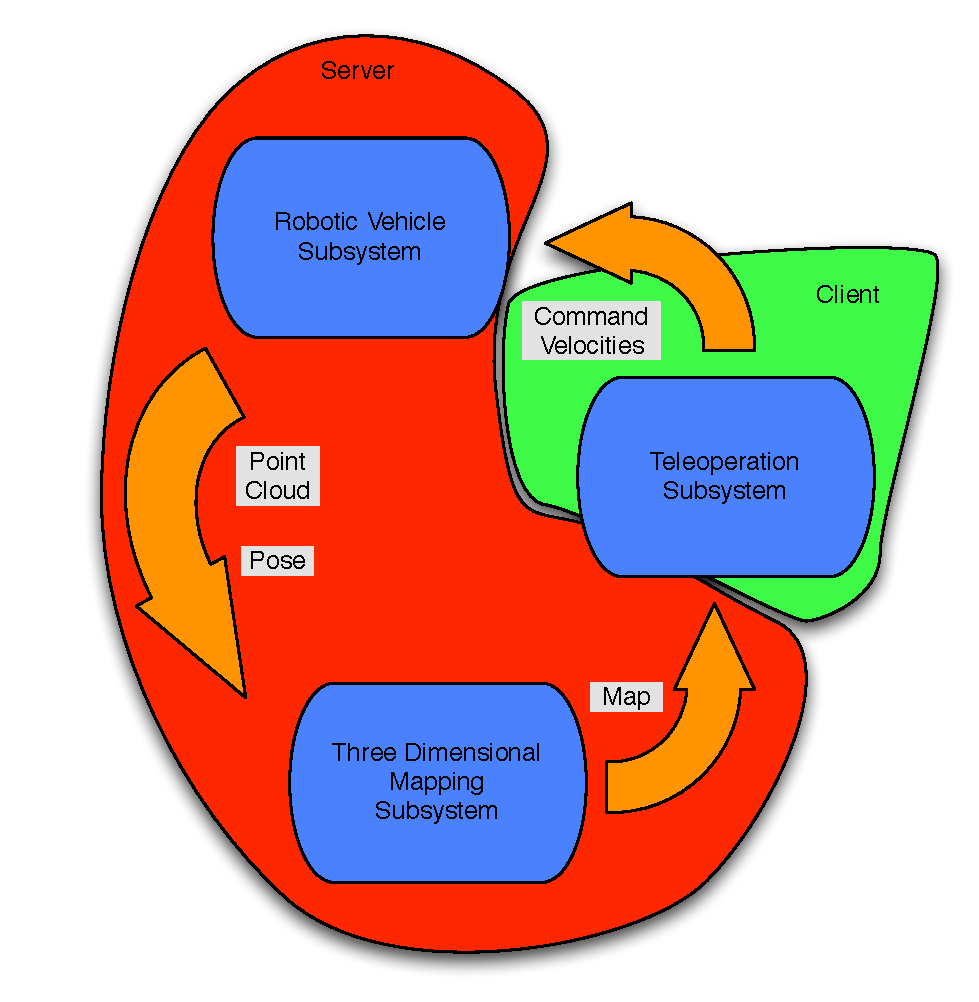
\includegraphics[width=5in,keepaspectratio]{subsystem.pdf}
  \caption{Subsystem Layout}
  \label{fig:subsystem}
\end{figure}

The above design assumes that all of the telemetry is processed by the mapping subsystem before being transmitted by the teleoperation subsystem.  It would be possible to transmit the raw telemetry to the teleoperator and then process it on the teleoperator's machine, but this was not the selected design pattern because the network bandwidth and latency was more valued than the processing power on the robotic vehicle.  This design attempts to meet the lowest common denominator by minimizing processing for the mapping and then transmitting the completed map, which can be much more concise than the raw telemetry.

By decoupling the three subsystems, replacing one implementation of a subsystem with another is much easier.  Because the interface of the robotic vehicle consist of one or more exteroceptive sensors, a proprioceptive pose solution, and a velocity command interface, the underlying robotic vehicle can be replaced with any robotic subsystem that can conform to that interface.  Similarly, the mapping subsystem can be replaced with any individual mapping system that takes the telemetry from the robotic vehicle and produces a map for the teleoperation subsystem.

\section{System Specification}
Breaking the subsystems down further provides implementation specific details.  Figure \ref{fig:system_diagram} shows the three subsystems in more detailed and more tightly integrated figure.  Though the interfaces are missing here the flow of information remains the same from the subsystem layout in Figure \ref{fig:subsystem}.

\begin{figure}[ht]
  \centering
  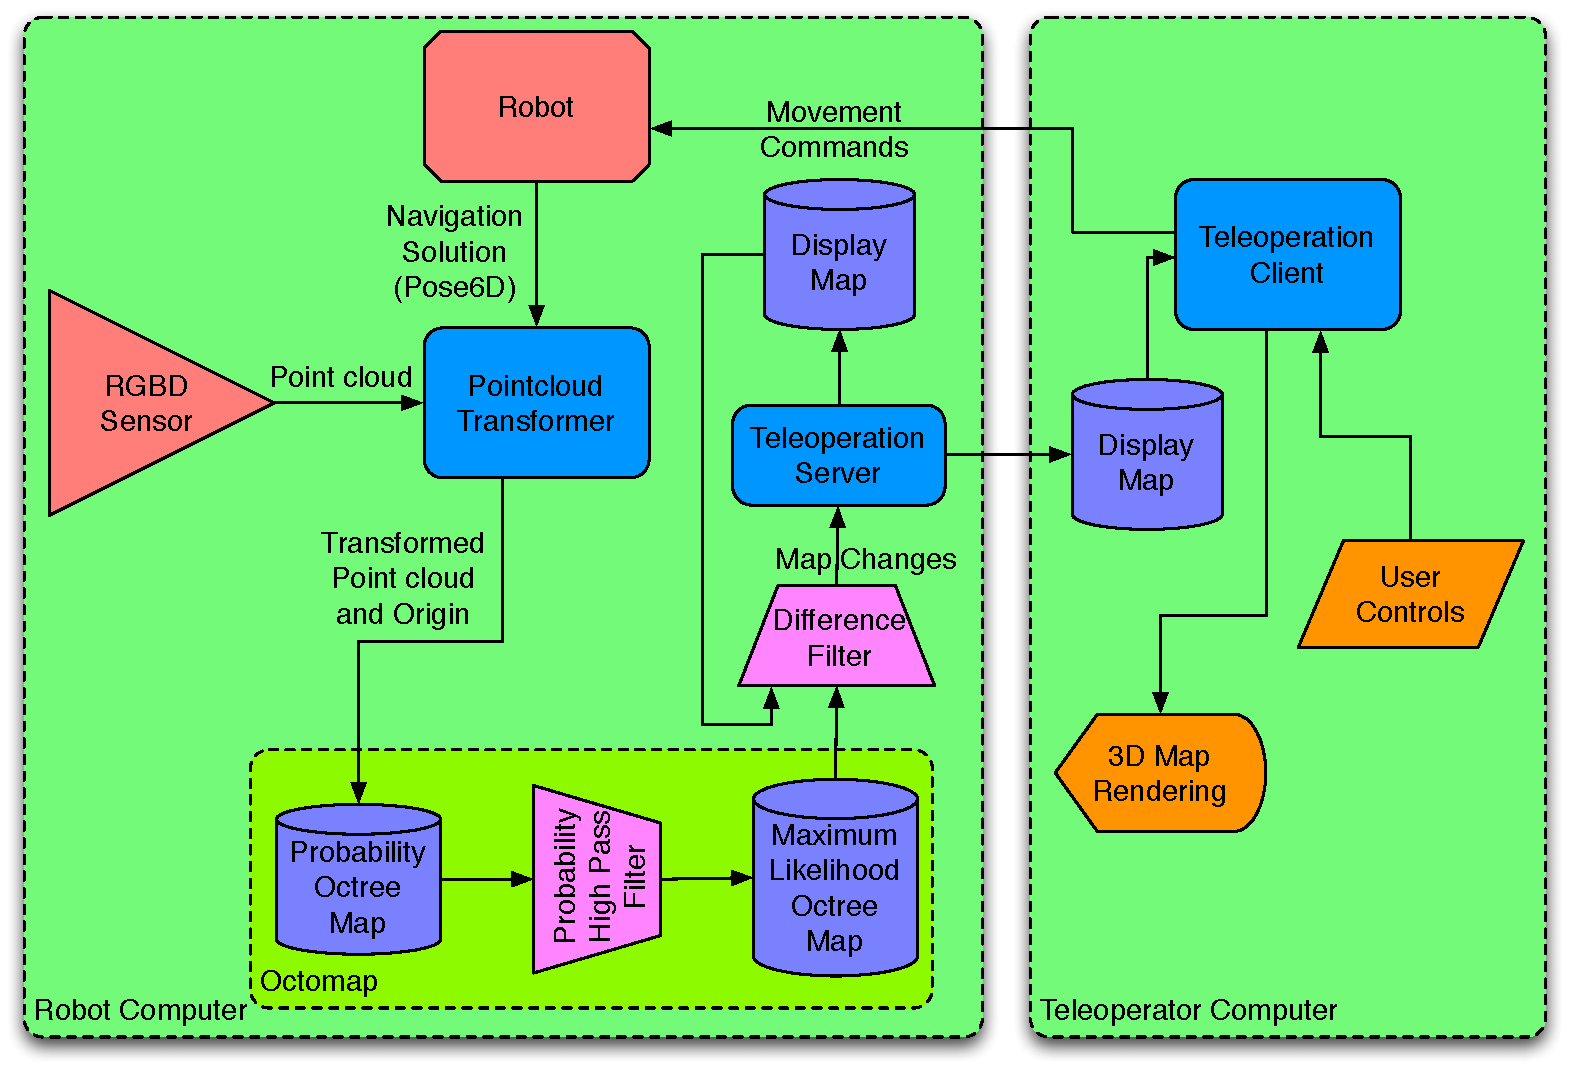
\includegraphics[width=6in,keepaspectratio]{system_diagram.pdf}
  \caption{Overview of System Design, the separation of activities by computer system are shown more clearly}
  \label{fig:system_diagram}
\end{figure}

As mentioned above, Figure \ref{fig:system_diagram} describes the overall system design.  The three dimensional data in the form of point clouds are collected from one or more sensors like the Microsoft Kinect.  These point clouds are combined with a navigation solution from the robotic base to transform the data points into a common map coordinate frame.  At this point the point clouds are inserted into the map using a probabilistic insertion method which is described in Chapter \ref{chap:3d_mapping}.  A maximum likelihood version of the map is generated and is stored in, what this work will refer to as, the server map.  The server map is now ready to be used in teleoperation, so the server map is subtracted from the current client's map resulting in map deltas (changes in the map).  The map deltas, or some smaller subset of the map deltas, are sent to the client and united with the current client map.  If all of the differences are sent, then the client map and the server map should then be synchronized, i.e. the client map is up-to-date.  Otherwise successive iterations of this process will eventually result in an up-to-date client map.  Simultaneously, input from the teleoperator is sent to the robotic vehicle to allow teleoperation.

The above description, or theory of operation, of the system makes references to several as yet undefined processes and design decisions.  There are more details on the Mapping and Teleoperation subsystems in Chapters \ref{chap:3d_mapping} and \ref{chap:teleoperation}, respectively.  The robotic subsystem and it aforementioned navigation solution are discussed in the next section and the Experimental Setup in Section \ref{sec:robotic_vehicle}.

% TODO: describe the Sick LMS151
\section{Robot Navigation}
A necessary component of the proposed teleoperation system is the ability for the robotic vehicle to provide an accurate pose estimate.  Because the system proposed does not rely on Iterative Closest Point (ICP) or feature mapping to combine successive point clouds, as in P. Henry, M. Krainin, and E. Herbst\cite{Henry2010}, the pose estimate from the robotic vehicle must be very accurate.  The trade off is that a much smaller amount of processing is required to generate the map, but the resulting quality of the map is sensitive to errors in the pose estimate.  Outdoor navigation systems like the Novatel SPAN system can provide $\sim$2 centimeters positional accuracy and 1/10th degree angular accuracy\cite{kennedy2006architecture}, which would be acceptable for mapping.  Indoor robots, like the experimental setup for this paper, require some other means of estimating its position in an arbitrary global coordinate frame.  The experimental system in this work uses an implementation of grid SLAM, which combines odometry from the wheel encoders with laser range finder data from a Sick LMS151.  An off-the-shelf SLAM library is used to get a high quality pose estimate indoors, and the library uses a grid based approach with particle filters to map and localize the environment.  The library is called the gmapping library\cite{grisetti2007improved}\cite{grisettiyz2005improving}, which is an open source library and can be found on openslam.org.  These navigation systems attempt give a high accuracy, drift resistant pose solution of the vehicle indoors.

%%%%%%%%%%%%%%%%%%%%%%%%%%%%%%%%%%%%%%%
%% Chapter: Three Dimensional Mapping
%%%%%%%%%%%%%%%%%%%%%%%%%%%%%%%%%%%%%%%

\chapter{Three Dimensional Mapping}\label{chap:3d_mapping}
As with the top level system design, other mapping solutions are analyzed before design begins.  In the following section a survey of past work is presented.

\section{Previous Work}
\label{sec:previouswork_3dmapping}
Recent work has been done to create three dimensional maps of the environment using octrees and a probabilistic insertion method that is well suited for robotic activities where noise is present in the data and uncertainty in the pose of the robot. A. Hornung, et. al. described and implemented this system, and it resulted in an open-source library called octomap.\cite{octomap} This work uses octomap as the octree mapping library, and a description of octomap and how it works is in Section \ref{sec:3dmapping}.

There are two main elements of the octomap research that are useful in a three dimensional teleoperation system.  First, the probabilistic method for adding new three dimensional information to the map is ideal for a system that needs to be updated continuously.  Uncertainty from the navigation solution will result in point clouds that are transformed incorrectly, and this causes inconsistencies and skews in the resulting map. The probabilistic manner in which the scans are inserted into the octree help to alleviate this inconsistency by allowing for some error in the point clouds in relation to the map. This error is further alleviated by the nature of the octree data structure because inserting the point clouds into the octree essentially results in a down-sampling of the original data to the resolution of the octree.

Second, limiting the query depth on the octree will effectively and efficiently down-sample the map.  The down-sampling allows for an adjustable quality level of the map being sent over the wire to match the available resources like network bandwidth and network latency.  Having adjustable quality is important because most teleoperation systems work over a wireless and unreliable communication layer, which often suffers from low data rates and large latencies.  An analogy can be drawn to how on-line video streaming services will adjust the compression of a video to accommodate the connection being used, but in these systems the main concern is bandwidth, not latency.

In addition to the work done by A. Hornung, et. al. with octomap, three dimensional mapping done specifically with RGB-D cameras from Primesense was done by P. Henry, M. Krainin, and E. Herbst\cite{Henry2010}.  In that publication they used alignment techniques like features with RANdom SAmple Consensus (RANSAC), Iterative Closest Point (ICP), and loop closure techniques to produce a very high quality map from the RGB-D data\cite{Henry2010}.  The mapping approach in this thesis differs in that it relies on other sensors and existing navigation solutions to provide accurate transforms for the points clouds in an attempt to make the system more processor efficient and run closer to real-time.  The work by P. Henry, M. Krainin, and E. Herbst still managed to perform the processing in a relatively small amount of time, but processing in that paper has not gotten to the speeds required for real-time teleoperation.

Very recent work by Microsoft using the Kinect has achieved real-time mapping with the Kinect in a project called KinectFusion\cite{izadi2011kinectfusion}.  Additional work has seen this technology demo reproduced using PCL and extended spatially\cite{whelankintinuous}.  This technique employs new methods for combining Kinect data on the Graphics Processing Unit of the video card in the computer.  This technology is very immature, but most likely will be a suitable replacement for the mapping system presented in this work.  The advantage to the mapping system presented in this work is that it requires less processing than the KinectFusion system.

\section{The Mapping Process}
\label{sec:3dmapping}
This section describes the process of combining the three dimensional data from the sensor and six dimensional poses from the robot base into three dimensional maps of the environment. As previously mentioned in Section \ref{sec:previouswork_3dmapping}, A. Hornung, et. al. have already shown that octrees combined with a probabilistic insertion method can provide a good solution when creating three dimensional maps. A portion of this section explains their work\cite{octomap} and how it is used in the teleoperation system described in this thesis work. The obvious first step of this process is obtaining the three dimensional data and the six dimensional pose of the robotic base from which the map is constructed, which is described briefly in Section \ref{sec:robotic_vehicle}.

\subsection{Transforming the Point Clouds}
Each time new data from the three dimensional sensor is received by the computer the data needs to be transformed into a common arbitrary global frame or `map' frame. Figure \ref{fig:transforms} shows a typical transformation tree for the robotic setup. The `base\textunderscore{}link' frame is commonly referred to as the vehicle frame. The transformation between the `map' frame and the `base\textunderscore{}link' frame represents absolute transformation given by the pose estimate of the robotic vehicle. The transformations between the `base\textunderscore{}link' frame and the `laser\textunderscore{}link' frame and the `camera\textunderscore{}link' frame are static geometric relationships and represent the position of the sensors on the robot chassis. When new point clouds are received they are in the `camera\textunderscore{}link' coordinate frame and need to be converted into the `map' coordinate frame as that is the corrected global frame in this situation.

\begin{figure}[ht]
  \centering
  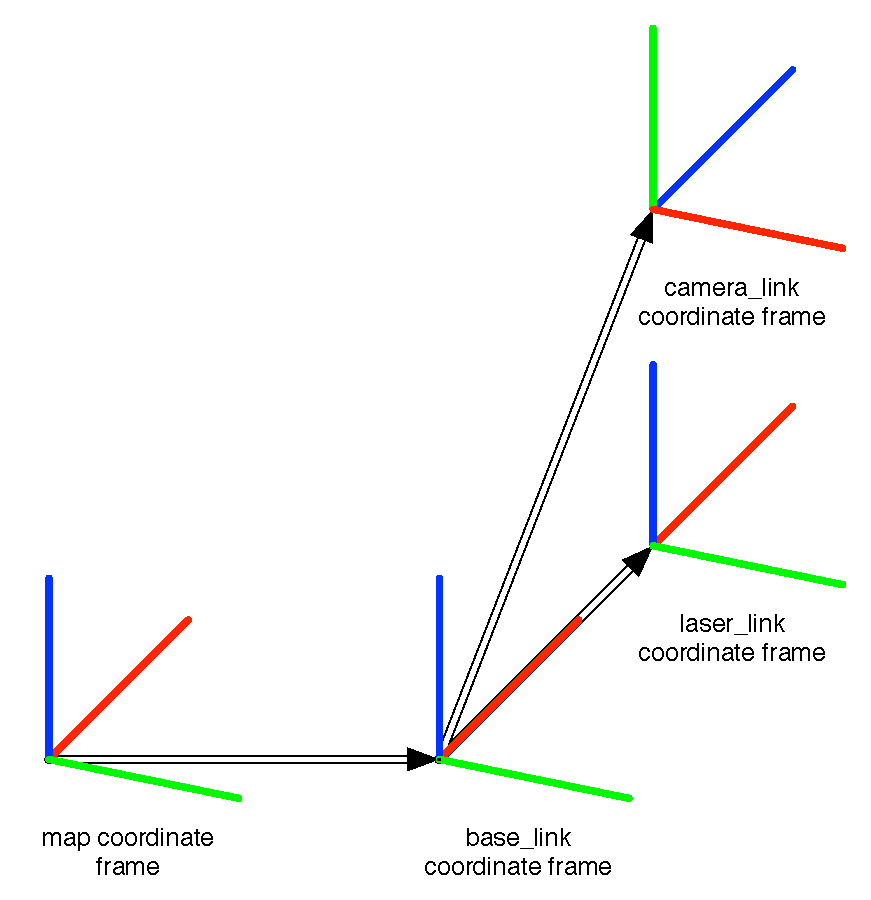
\includegraphics[width=4in,keepaspectratio]{transforms.pdf}
  \caption{Typical Coordinate Transform Tree}
  \label{fig:transforms}
\end{figure}

In order to transform the point clouds into the global coordinate frame, each point in the point cloud must be transformed into the global coordinate frame.  Each point is represented by the homogeneous vector in Equation (\ref{eq:point}).

\begin{equation} \label{eq:point}
\left[ \begin{array}{c} x \\ y \\ z \\ 1 \end{array} \right]
\end{equation}

The points are transformed using the homogeneous transform matrix\cite{lavalle2006planning}, defined in Equation (\ref{eq:transform_matrix}).

\begin{equation} \label{eq:transform_matrix}
\left[ \begin{array}{cccc} \cos \psi \cdot \cos \beta  & \cos \psi \cdot \sin \beta \cdot \sin \gamma \; -\; \sin \psi \cdot \cos \gamma  & \cos \psi \cdot \sin \beta \cdot \cos \gamma \; +\; \sin \psi \cdot \sin \gamma  & x_{t} \\ \sin \psi \cdot \cos \beta  & \sin \psi \cdot \sin \beta \cdot \sin \gamma \; +\; \cos \psi \cdot \cos \gamma  & \sin \psi \cdot \sin \beta \cdot \cos \gamma \; -\; \cos \psi \cdot \sin \gamma  & y_{t} \\ -\sin \beta  & \cos \beta \cdot \sin \gamma  & \cos \beta \cdot \cos \gamma & z_{t} \\ 0 & 0 & 0 & 1 \end{array} \right]
\end{equation}

In the homogeneous transform matrix $\gamma$ is Roll about the $x$-axis, $\beta$ is pitch about the $y$-axis, and $\psi$ is Yaw about the $z$-axis.  $x_{t}$, $y_{t}$, and $z_{t}$ are the translational components of the transform matrix.

By multiplying each of the points in the point cloud by this transform matrix, the entire point cloud is transformed into the global coordinate frame and is ready to be inserted into the map.

\subsection{Inserting New Data}
% TODO: describe ray tracing
Once the point cloud data has been transformed into the global coordinate frame, the data needs to be added to the map. As previously mentioned, inserting data is done by the octomap library, but the process is described here for clarity. The underlying data structure for this map is an octree where each leaf has a probability of occupation. The octree is in effect a three dimensional occupancy grid with octree storage where each leaf of the tree is a voxel, also known as grid cell, in the grid. The transformed data and the origin of the sensor in the global coordinate frame are required for the insertion. The insertion method starts by iteratively ray tracing from the origin of the sensor to each data point in the point cloud.  For each voxel that the ray trace passes through the probability of occupation of that voxel is decreased by a given amount. For the voxel that the ray trace ends in, the probability of that voxel being occupied is increased by a given amount. In this way several points must fall into a voxel to have voxel considered to be occupied, and allows for fringe voxels, caused by noise, to be cleared by additional new data.

\begin{figure}[ht]
  \centering
  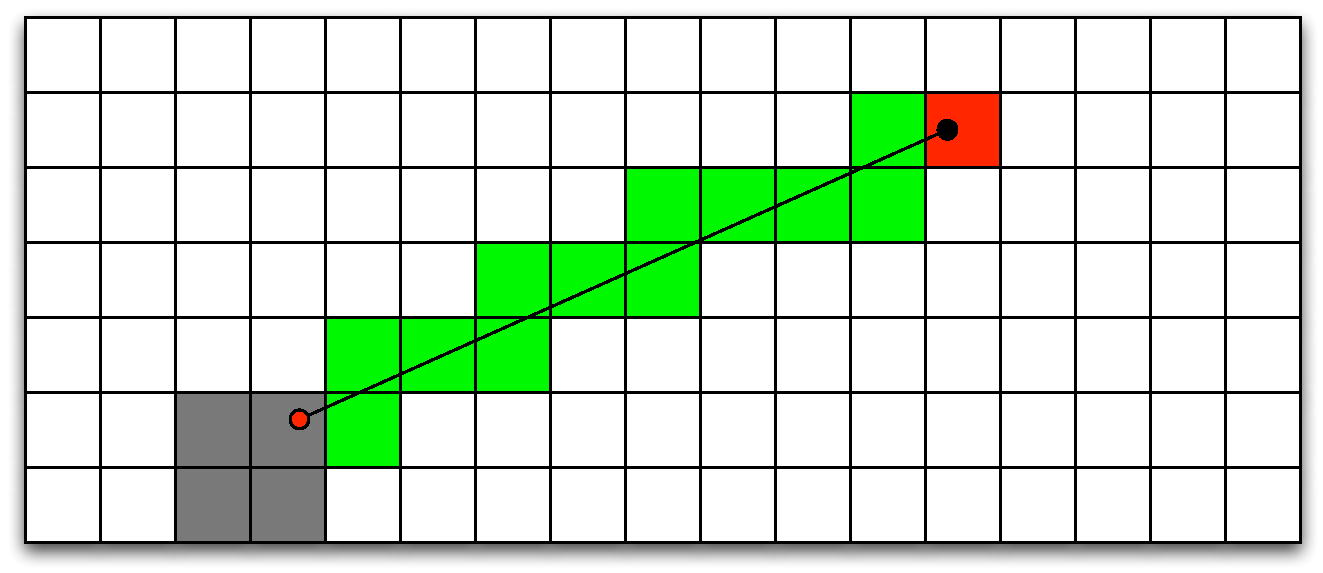
\includegraphics[width=5in,keepaspectratio]{raytrace.pdf}
  \caption{Two Dimensional Example of Voxel Ray Tracing}
  \label{fig:voxel_raytrace}
\end{figure}

Figure \ref{fig:voxel_raytrace} shows this process in a two dimensional example where the gray voxels are the robot, the red dot is the sensor origin, the black dot is the point from the point cloud, the green voxels are having their occupancy decreased, and the red voxel is having its occupancy increased. This method of voxel ray tracing is originally proposed by Amanatides, J. and Woo, A., and is referenced in the octomap paper\cite{amanatides1987fast}.

\section{Sources of Error During Three Dimensional Mapping}
With this approach to three dimensional mapping, map quality can be adversely affected by several different sources of error, including the uncertainty in the pose estimate of the robotic vehicle, random and systematic error in the three dimensional data, and systematic errors due to timing and geometric misalignment.  Figure \ref{fig:slamvsoctree} shows the resulting octree map with the map from the Simultaneous Localization and Mapping (SLAM) algorithm, which is good enough in this instance to be considered truth. The octree map generally lines up with the SLAM map but has a lot of areas where the result is less than desirable.

\begin{figure}[ht]
  \centering
  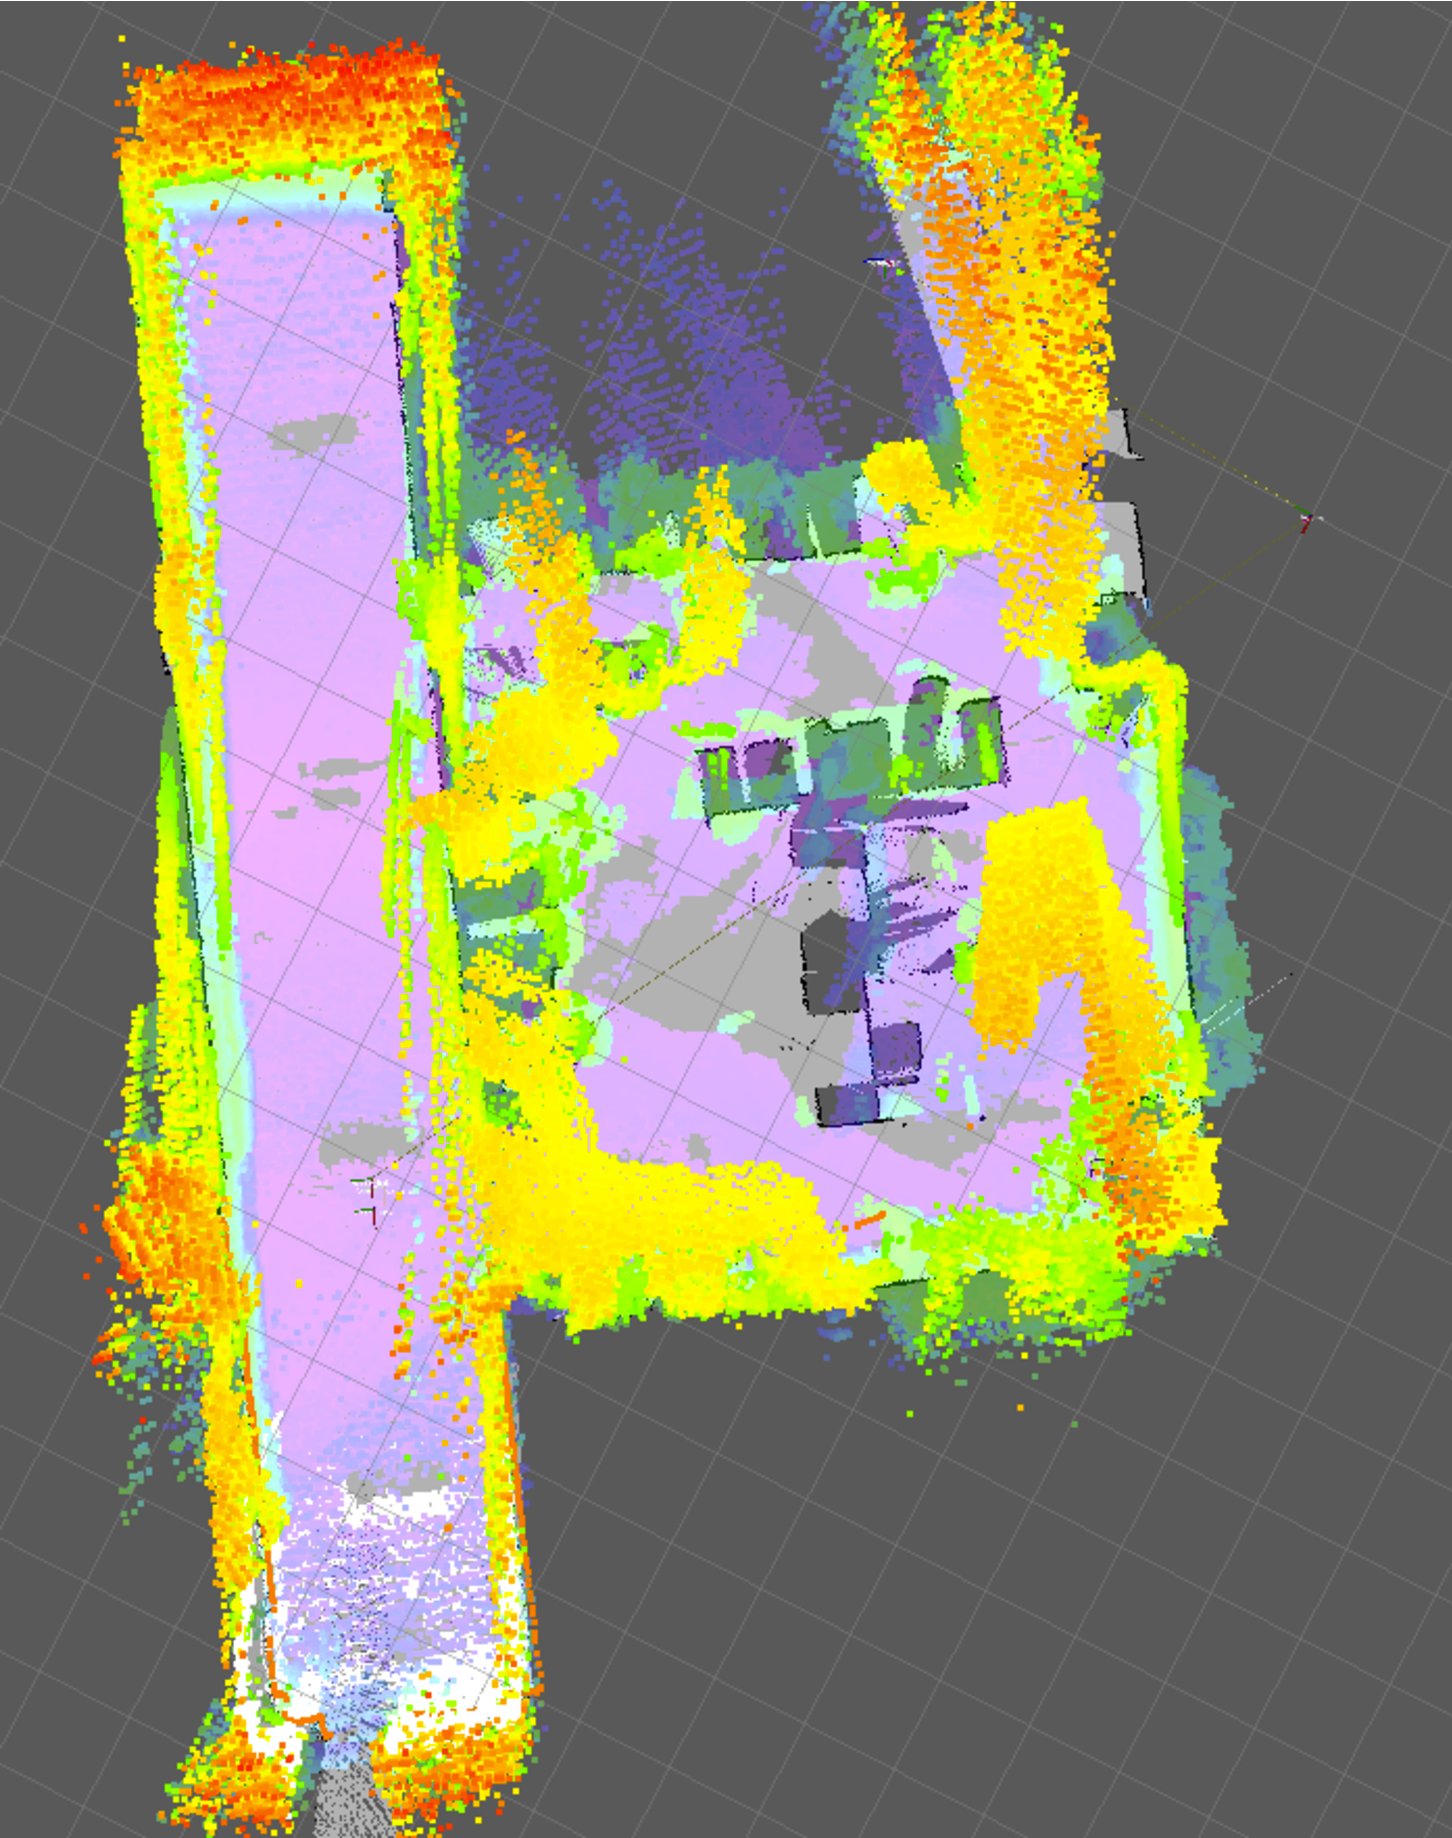
\includegraphics[width=4in,keepaspectratio]{slamvsoctree.pdf}
  \caption{A top down, orthographic view of a three dimensional map generated from Kinect data with a map created by the SLAM library}
  \label{fig:slamvsoctree}
\end{figure}

\subsection{Vehicle Pose Uncertainty}
\label{sec:uncertainty}
A major component of the error introduced in mapping with this system is the vehicle pose uncertainty.  In most robotic systems, and in the system presented in this thesis, the pose estimate is a blend of multiple sensors, some that drift and some that bound error growth.  In this case the pose estimate will have a cycle where the error grows until it is sharply bound by a measurement update.  In the system in this thesis, bounding occurs when a SLAM update occurs.  The SLAM algorithm provides updates to the pose of the vehicle at about 1 Hz, and between these updates the integrated wheel odometry is used to provide poses.  The integrated wheel odometry quickly diverges from the true path of the vehicle and the uncertainty grows quickly, especially when turning in place where the non-linear effects of slip are neglected in the integration of the encoders.  Therefore the uncertainty grows and then is sharply snapped back on a SLAM update.  This effect can be seen in Figure \ref{fig:uncertainty}, where the misalignment of the laser data, and the map becomes obvious.  After a SLAM update the pose estimate is much better.  Just before a SLAM update the pose is generally at its highest uncertainty, so inserting a point cloud at this point in time would produce the worst results for mapping.

\begin{figure}[ht]
  \centering
  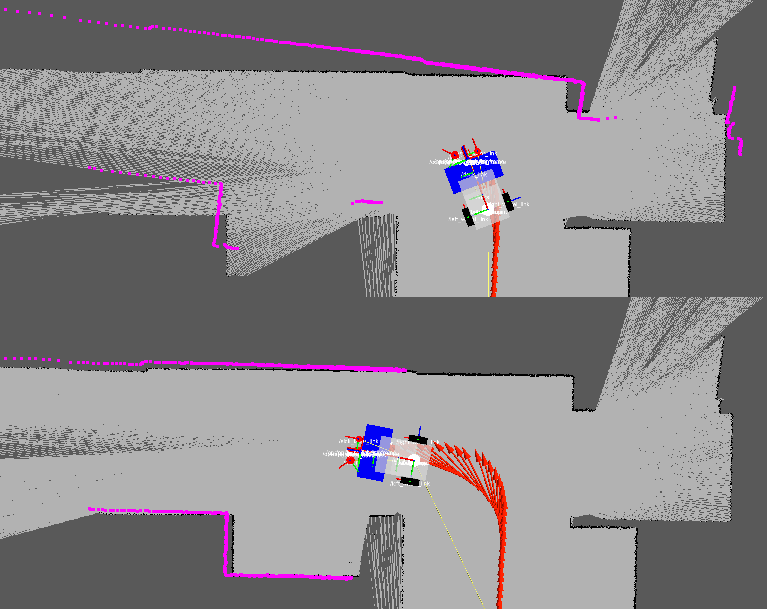
\includegraphics[width=6in,keepaspectratio]{uncertainty.png}
  \caption{Integrated wheel odometry diverging from the pose provided by SLAM when turning}
  \label{fig:uncertainty}
\end{figure}

Another problem that comes up in the mapping process is that inserting point clouds into the octree map is computationally expensive.  The computation required is affected by the density of the point cloud data and the resolution of the map.  Some sensors, like the Kinect and Xtion Pro Live, produce this point cloud data at high rates, which can be as high as thirty hertz.  Due to the computational limitations and the high rate of speed of the data, many of the point clouds have to be dropped.  This is not necessarily a problem for mapping in the system presented here, because of the rate of the point cloud data and the speed of the robotic vehicle, 1-2 meters per second, much of the point cloud data is redundant.

A practical solution to both of these problems is to opportunistically select point clouds to insert.  In this system only point clouds that comes after SLAM updates are inserted.  Timing is a critical component at this stage, it is important to match SLAM transform timestamps to point cloud timestamps as closely as possible to avoid further misalignment in the map.

%TODO: compare opportunistic insertion to non

Another solution to this problem is to simply produce a better navigation solution.  Though not pursued in this work, combining the odometry with an Inertial Measurements Unit (IMU) or simply a yaw rate gyro with a Kalman Filter would likely reduce the error from the grow-bound cycle in the mapping process.  Point clouds would still need to be throttled, but which point clouds used would no longer matter as much.

\subsection{Sensor Random Error}
Another less prominent source of error is the random error in RGB-D cameras like present in the Kinect and the Xtion Pro Live.  Three sources of error in the this data are: loss of precision on depth measurements at greater distances, discretization error on depth measurements, and decreased density of data at greater distances.  The most prominent of these error sources is the variance in the depth measurement.  Khoshelham, K. showed that the random error in the depth of the Kinect data could be modeled from the theoretical principal of the depth sensor\cite{khoshelham2011accuracy}.  In the paper by Khoshelham, K., they show theoretically and experimentally that the depth variance at 4 meters is about 5 centimeters.  This variance changes over distance, with smaller distances yielding more precise measurements than at greater distances.

\begin{figure}[ht]
  \centering
  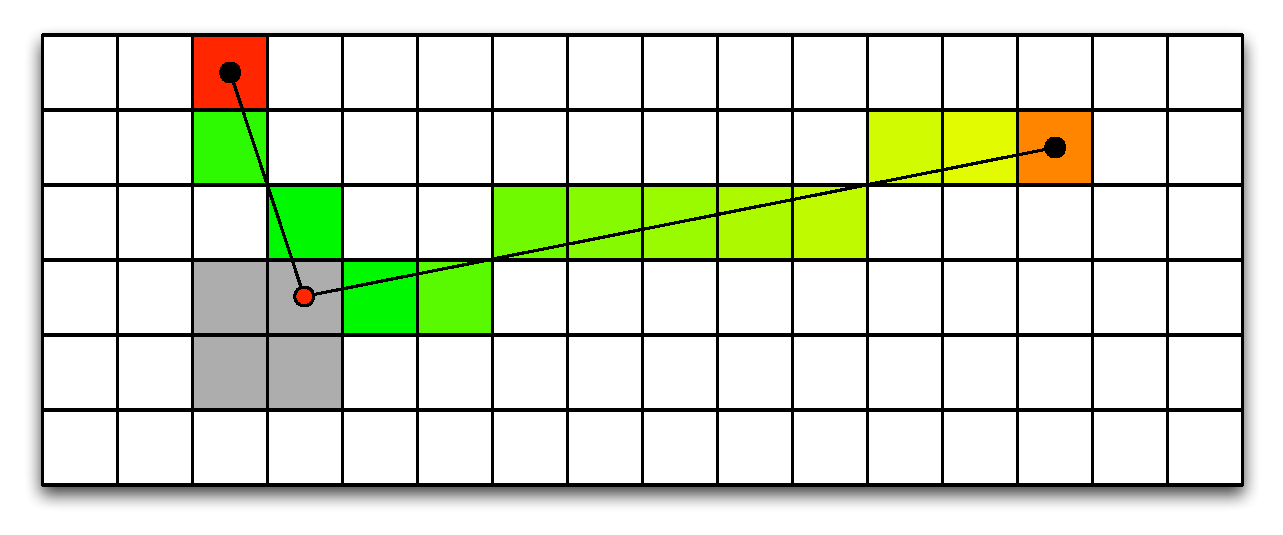
\includegraphics[width=6in,keepaspectratio]{variable_hit_miss.pdf}
  \caption{This figure demonstrates the variable hit and miss values used during ray tracing.}
  \label{fig:variable_hit_miss}
\end{figure}

In order to help minimize this error, a practical solution might be to ignore data that is further than 3 or 4 meters as the variance grows quite large.  The system in this work, however, makes a small modification to the method of insertion used by octomap.  Instead of having a constant hit and miss value for ray tracing each point in each point cloud, the hit and miss values change based on the distance to the origin of the sensor.  In this way data that is further from the sensor, especially greater than 3 or 4 meters, is less likely to make a voxel occupied and less likely to clear an occupied voxel.  The variable hit and miss values allow the system to incorporate data past 4 meters, but also takes into account the decreased precision.

Figure \ref{fig:variable_hit_miss} shows the effect of long and short ray casts with the above proposed changes.  In the figure the values are varied linearly by distance from the sensor origin, but in practice the system uses a quadratic scaling of the hit and miss values.  Additionally, the scaling does not start until 3 meters from the sensor.  These two changes from the simple linear scaling method reflect the fact that the data under 4 meters is quite good, and the data degrades non-linearly at greater distances.  The results of this tactic on mapping are noticeable in specific situations, but overall improvements are marginal compared to the mapping error induced by errors in the navigation solution.

%%%%%%%%%%%%%%%%%%%%%%%%%%%%%%%%%%%%%%%
%% Chapter: Teleoperation
%%%%%%%%%%%%%%%%%%%%%%%%%%%%%%%%%%%%%%%

\chapter{Teleoperation}\label{chap:teleoperation}
While the three dimensional map is being continuously generated, the client needs to be updated regularly so that the teleoperator has up-to-date telemetry from which to make decisions about the commands to send to the robotic vehicle. This step is where the application of the three dimensional mapping to teleoperation occurs. Periodically the probability octree that represents the current best guess as to the occupancy of the environment is converted to a maximum likelihood tree.  This maximum likelihood tree is compared to the client's map of the environment.  The differences are sent over the wire to the client, where the differences are united with the current client map, effectively updating the map used for visualization.  Iterating these actions in parallel with the three dimensional mapping process allows for timely updates and a gracefully degrading difference model based on available bandwidth.

\section{Maximum Likelihood Representation}
The point clouds are initially inserted into an occupancy probability octree where the leaves contain the probability of occupation, but this representation is large and not suited for processing and transmitting the map over the wire in a low bandwidth and/or latent network. The map is therefore periodically transformed into a maximum likelihood version of the probabilistic octree. This transformation is performed by applying a probability high pass filter on the probabilistic octree, where the voxels that are most likely occupied are seen in the transformed octree. The maximum likelihood octree is much more compact because each leaf can be represented with exactly two bits each\cite{octomap}.  Two bits per leaf allows for four unique states for each leaf - of which three are utilized, occupied, unoccupied, or unknown.

\section{Map Streaming}
Once the map is in the maximum likelihood tree format, the map needs to be transmitted to the client. In some cases, however, there is more data to send than there is bandwidth available. In these cases a lower resolution version of the map differences can be sent and more detailed differences can be sent in the future when more bandwidth is available.

\subsection{Octree Set Difference}
The first step in synchronizing the server and client octrees is to detect what has changed since the last update. In order to determine this, the client octree is set differenced with the server octree which yields the changes in the server from a previous point in time. In order to find the set difference between the two octrees Algorithm \ref{alg:octree_diff} is used. This algorithm is a simple element-wise difference and can be considered a volumetric difference.

\begin{algorithm}
\caption{Algorithm for Pairwise Difference of Octrees}
\label{alg:octree_diff}
\begin{algorithmic}
  \STATE \COMMENT {$O_0$ is the server occupancy tree}
  \STATE \COMMENT {$O_1$ is the client occupancy tree}
  \STATE \COMMENT {$d$ is the set difference}
  \FORALL{leafs in $O_0$}
    \IF {leaf not in $O_1$}
      \STATE $d\gets leaf$
    \ENDIF
  \ENDFOR
  \RETURN $d$
\end{algorithmic}
\end{algorithm}

\subsection{Bandwidth Adjustment Algorithm}
Once the differences have been determined, the differences need to be sent over the network to the client computer to be united with the current client map. If not enough bandwidth is available, the differences can be reduced by differencing the two octrees at a lower resolution. The lower resolution versions of the trees can be obtained by limiting the depth of the query into the octree.  For example, if the leaf size of the octree is 2 centimeters, then reducing the query depth by one will result in a subtree with leaves, 4 centimeters in size.  This phenomenon is demonstrated in a map of the Shelby Center at Auburn University by Figure \ref{fig:treedepth}.  The visualization in Figure \ref{fig:treedepth} was done using octovis\cite{octomap}, which is part of octomap.

\begin{figure}[ht]
  \centering
  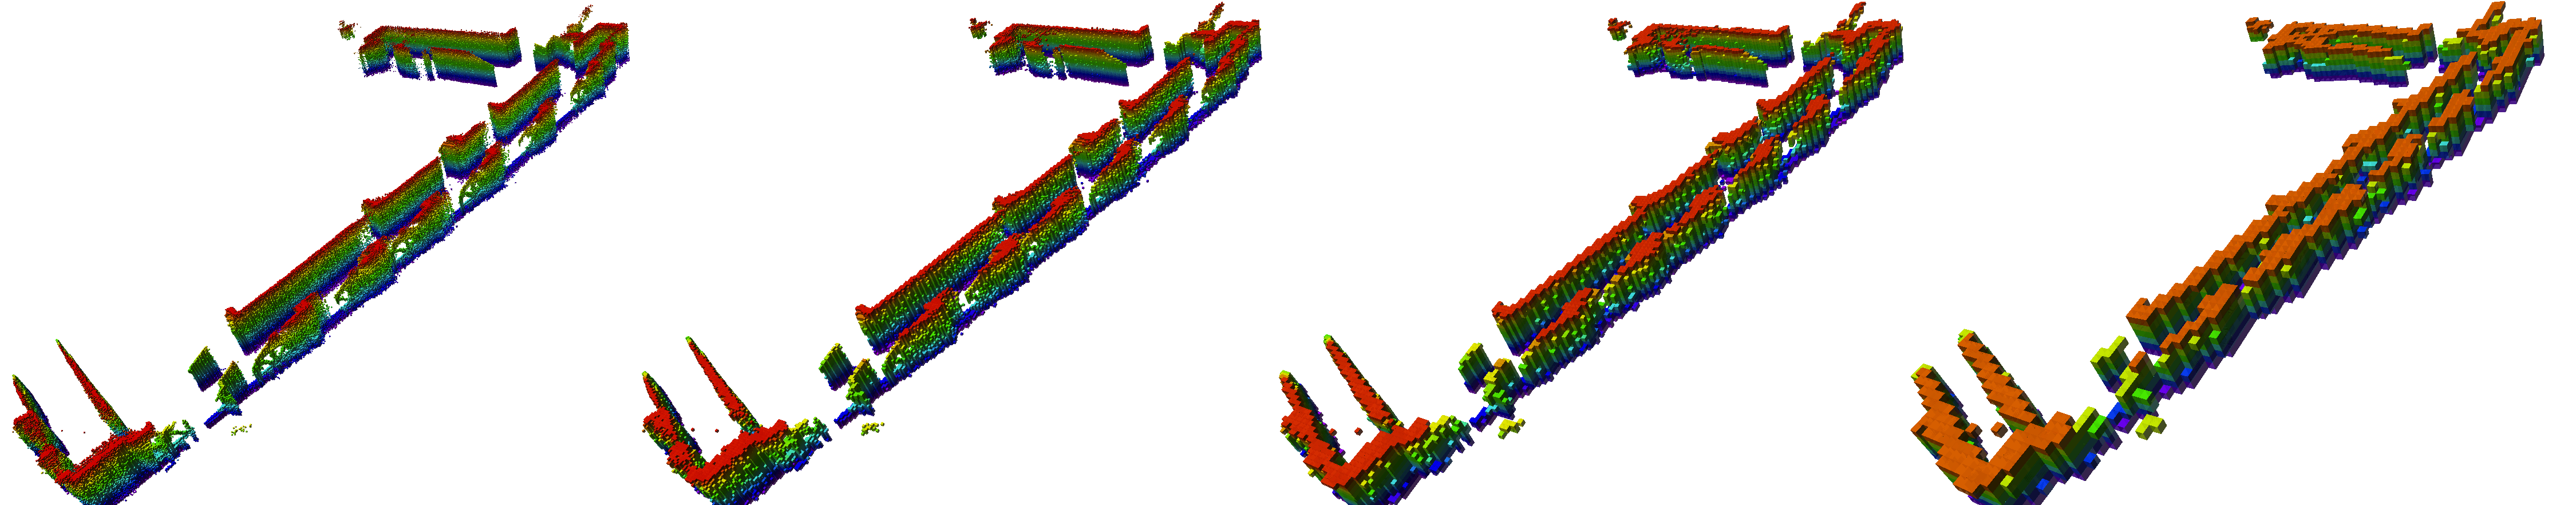
\includegraphics[width=6in,keepaspectratio]{ShelbySE_2f_combined_octovis.png}
  \caption{Partial map of a hallway showing the effect of limiting the query 
           depth.  From left to right the resolution is 0.05m, 0.1m, 0.2m,
           and 0.4m.}
  \label{fig:treedepth}
\end{figure}

The algorithm for selecting the depth is proposed in Algorithm \ref{alg:bandwidth} and simply continues to degrade the resolution until enough bandwidth is available to transmit or until there resolution cannot be degraded further.

\begin{algorithm}
\caption{Algorithm for Determining Difference Depth}
\label{alg:bandwidth}
\begin{algorithmic}
  \STATE \COMMENT {$O_0$ is the server map octree}
  \STATE \COMMENT {$O_1$ is the client map octree}
  \STATE \COMMENT {$d$ is the set difference}
  \STATE \COMMENT {$B_d$ is the bandwidth required to transmit the diff}
  \STATE \COMMENT {$B_a$ is the available bandwidth}
  \STATE \COMMENT {$T_u$ is the update period in seconds}
  \STATE \COMMENT {$h_{max}$ is the maximum size of a leaf to be transmitted}
  \STATE $i\gets 0$
  \REPEAT
    \STATE $O_0 \prime = depth(O_0,height(O_0)-i)$
    \STATE $O_1 \prime = depth(O_1,height(O_1)-i)$
    \STATE $d = O_0 \prime \cup O_1 \prime $
    \STATE $B_d = size(d) / T_u$
    \STATE $B_a = currentAvailableBandwidth()$
    \STATE $i = i + 1$
  \UNTIL {$B_d\le B_a \| resolution(i) \ge h_{max}$}
  \RETURN $d$
\end{algorithmic}
\end{algorithm}

The depth function simply returns a subtree of the given tree at the given height, and the height function gives the height of the specified tree.  The resolution function simply returns the dimension of a leaf at the given level.  The current available bandwidth function could be implemented in several ways, which has been covered in the literature\cite{prasad2003bandwidth}. The principle behind the bandwidth estimation includes metrics like round-trip-time, average delay, packet loss, and throughput to determine the bandwidth currently available.  In this thesis testing, as discussed in Chapter \ref{chap:experiments}, the bandwidth was artificially controlled to exercise this component of the system.  Artificially controlling the bandwidth used by the mapping system will also allow for quality of service to be enforced.  Quality of service would allow the system to prioritize things like teleoperation commands, video, or other telemetry over the map update.

\subsection{Octree Set Union}
The final stage of synchronizing the server and client octrees is to unite the differences with the client octree. This algorithm is just a simple union operation and can be performed by simply inserting every voxel of the differences into the client map using the normal octree insertion method as in \cite{meagher1982geometric}.

\section{Visualization}
The purpose of mapping the environment and streaming that map to the client is so that the teleoperator might gain some improvement of control when teleoperating the robotic vehicle.  In addition to the map being sent to the client, the position of the robotic vehicle in the map coordinate frame must be sent to the client as well.  With these two pieces of information the visualization of the vehicle in the three dimensional environment is possible.

\subsection{Rviz}
Rviz\cite{rviz} is a visual debugging tool provided by the Robotic Operating System (ROS)\cite{quigley2009ros}.  ROS is used at large in the experimental implementation of this system.  Rviz provides interfaces to visualize generic data types commonly found in robotics, like point clouds, laser scans, odometry, transforms, and others.  In addition to these generic data formats, rviz allows for more general drawing programmatically using primitive shapes like cylinders, spheres, boxes, and points.  More advanced shapes and custom shapes are also allowed.  These shapes can be seen in Figure \ref{fig:rviz_shapes}.

\begin{figure}[ht]
  \centering
  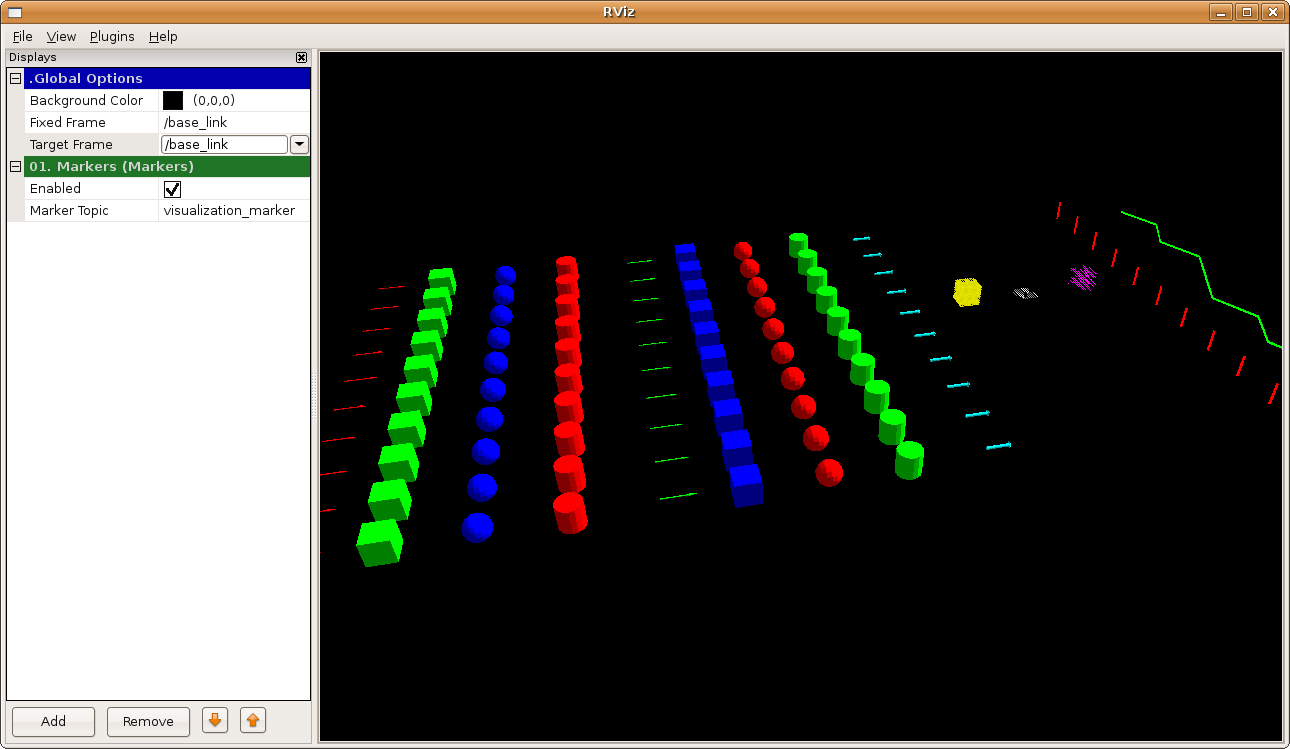
\includegraphics[width=6in,keepaspectratio]{rviz_shapes.png}
  \caption{Demo of drawing types in rviz\cite{rviz_shapes}}
  \label{fig:rviz_shapes}
\end{figure}

Since the underlying system is already using ROS and rviz provides methods for drawing custom three dimensional information, rviz was chosen as the basis for the visualization system.

\subsection{Rendering the Map}\label{sec:rendering_the_map}
In order to visualize or render the map using rviz, the map data must be put into a format that rviz supports.  There is no standard data type that satisfies the display of an octree.  Though each leaf of the octree could be represented as a point in a point cloud, each leaf also can have different sizes - i.e. not all leaves in the octree are the lowest depth of the tree.  Therefore custom drawing tools are required for drawing the octree correctly.

For efficiency in drawing, one of the custom drawing types is a `cube list', in contrast to just a `cube' drawing type.  In a cube list, a single message is sent to rviz which is of type `cube list' and has an array of positions and colors for each cube in the list.  Sending cube lists is far more efficient than sending a message to rviz for each leaf in the octree.  Each cube in a cube list, however, must be the same size.  Therefore, a cube list must exist for each level of the octree.

\begin{algorithm}
\caption{Algorithm for Drawing an Octree in Rviz}
\label{alg:octree_rviz}
\begin{algorithmic}
  \STATE \COMMENT {$O$ is the client map octree}
  \STATE \COMMENT {$cubelists$ is an array of leaf sets})
  \FOR{$leaf$ in $leaves(O)$}
    \STATE $cubelists\{size(leaf)\} = cubelists\{size(leaf)\} \cap leaf$
  \ENDFOR
  \FOR{$i=0$ to $height(O)$}
    \STATE $sendCubeList(cubelists\{i\}, size(cubelists\{i\}\{0\}))$
  \ENDFOR
\end{algorithmic}
\end{algorithm}

The algorithm for drawing an octree in rviz is displayed above in Algorithm \ref{alg:octree_rviz}.  In the algorithm the $leaves$ function returns an array of the leaves in the given octree, the $size$ function returns the dimensions of the voxel represented by a given leaf, and the $sendCubeList$ function sends the given set of leaves to rviz to be rendered at the given size.  This algorithm sorts the leaves of the octree into sets by height.  Then each set of leaves can be sent as one `cube list' of the appropriate size for that height to be rendered in rviz.

\subsection{Coloring the Octree}
When rendering the octree, a few options are available on how to color them.  One obvious option is to make all the leaves the same flat color.  However, a single color makes it difficult to see the three dimensional structure, so this color method is not used.  Another option is to color the voxels of the octree by height in the global coordinate frame.  The height map coloring gives some context to the voxels, where the lowest to the ground voxels will be one color and voxels near the ceiling will be a different color.  The height map coloring is the most effective method of rendering the voxels such that the teleoperator can understand the three dimensional structure.

Another option is to color the voxels by the color they would have in the real environment.  Per point coloring requires that the system, like the Kinect or Xtion Pro Live, provides color per point in the incoming point clouds.  This information is stored in the octree as an average of the colors of points that raytraced to each leaf.  This representation can add a more photo realistic quality to the environment for the teleoperator but consumes additional bandwidth and does not render well when the map is at a low resolution, therefore the height color map was chosen as the standard for the experiments.

\section{Teleoperator Input}
The final responsibility of the teleoperation subsystem is to collect the input from the teleoperator and transmit the input to the robotic vehicle.  Capturing the input is achieved using a Human Interface Device (HID) like a gamepad or a joystick.  In addition to a gamepad or joystick, a more vehicle like system could be used like a steering wheel and pedals.  The input from one of these devices is mapped to linear and angular velocities that are appropriate for the vehicle being teleoperated.  These linear and angular velocities are then sent to the robotic vehicle when they are executed by that subsystem.

%%%%%%%%%%%%%%%%%%%%%%%%%%%%%%%%%%%%%%%
%% Chapter: Latency Reduction
%%%%%%%%%%%%%%%%%%%%%%%%%%%%%%%%%%%%%%%

\chapter{Latency Reduction}\label{chap:latency_reduction}
One of the largest factors in a teleoperator's ability to control a vehicle effectively is how much latency is in the teleoperation system.  Previous work has shown that as latency increases the teleoperator's average speed goes down, and the ability to navigate around obstacles decreases\cite{photo_real}\cite{kaber2000effects}.  In this chapter a method for reducing the effects of latency is described.  By using a model of the robotic vehicle and the control input from the teleoperator, the position of the robotic vehicle can be estimated in the three dimensional environment.  This gives the teleoperator immediate visual feedback about their control input even before the robotic vehicle receives the commands and even longer before the telemetry about the robotic vehicles movement is received by the teleoperator's computer.

\section{Latency}
The transmission latency experienced in a teleoperation system can be described as two parts, the send latency and the receive latency.  The send latency is the time it takes for information generated on the teleoperator computer to be sent to the robotic vehicles computer.  The receive latency is the time for the reverse to occur, i.e. for data generated on the robotic vehicles computer to be sent to the teleoperator computer.  In most networks the latency to and from a remote network node are about the same, meaning that round trip time (RTT) is split even between sending and receiving.  The RTT being split evenly is true on average, but the latency, especially over reliable wireless networks, varies randomly with environmental conditions.  Even over short periods the RTT can vary quite a bit, but in systems that have sufficient bandwidth and good signal strength this variance is minimal.  It is also important to note that when referring to RTT latency the time spent processing on the remote machine is not included, which is why it is often broken into sending and receiving latencies.

In addition to the transmission latency there exists processing latency on both sides of the teleoperation system.  On the robotic vehicle system there is a latency between when something physically occurs and when the data indicating the change is sent to the teleoperator.  In the case of a camera there is a delay between when the image is captured and when it is sent caused by processing the image and preparing or packaging it for transmission.  This is more pronounced when the data being transmitted is aggregated data.  For instance, when new three dimensional data is received, there is latency incurred while inserting the new data into the map before the map is then packaged and transmitted to the teleoperator computer.  On the teleoperator computer there is overhead due to transmitting data to the robotic vehicle computer, but the commands sent are usually small and this latency is insignificant.  If the teleoperator computer, however, needed to transmit a map to the robotic vehicle computer for some reason, then this effect would be greater.

\section{Reducing Latency}
One method for reducing the effects of latency while teleoperating the robotic vehicle is to provide the teleoperator an estimate of the robot vehicles pose based on the teleoperators input.  In order to create this estimate, the teleoperator computer uses the latest available robot vehicle position in conjunction with the user input since that latest position to simulate the motion of the robotic vehicle on the teleoperator computer interface.  Motion is simulated over a period of time bounded by the time stamp of the latest robot vehicle pose and the current time.  The simulation is run continuously at a constant rate incorporating new user input as time moves forward, but the entire simulation must be rerun when new telemetry from the robot is received.  This adds a constraint on the simulation look ahead time, in that the simulation cannot accurately predict the vehicle position into the future because there is no user input for the future.

\begin{figure}[ht]
  \centering
  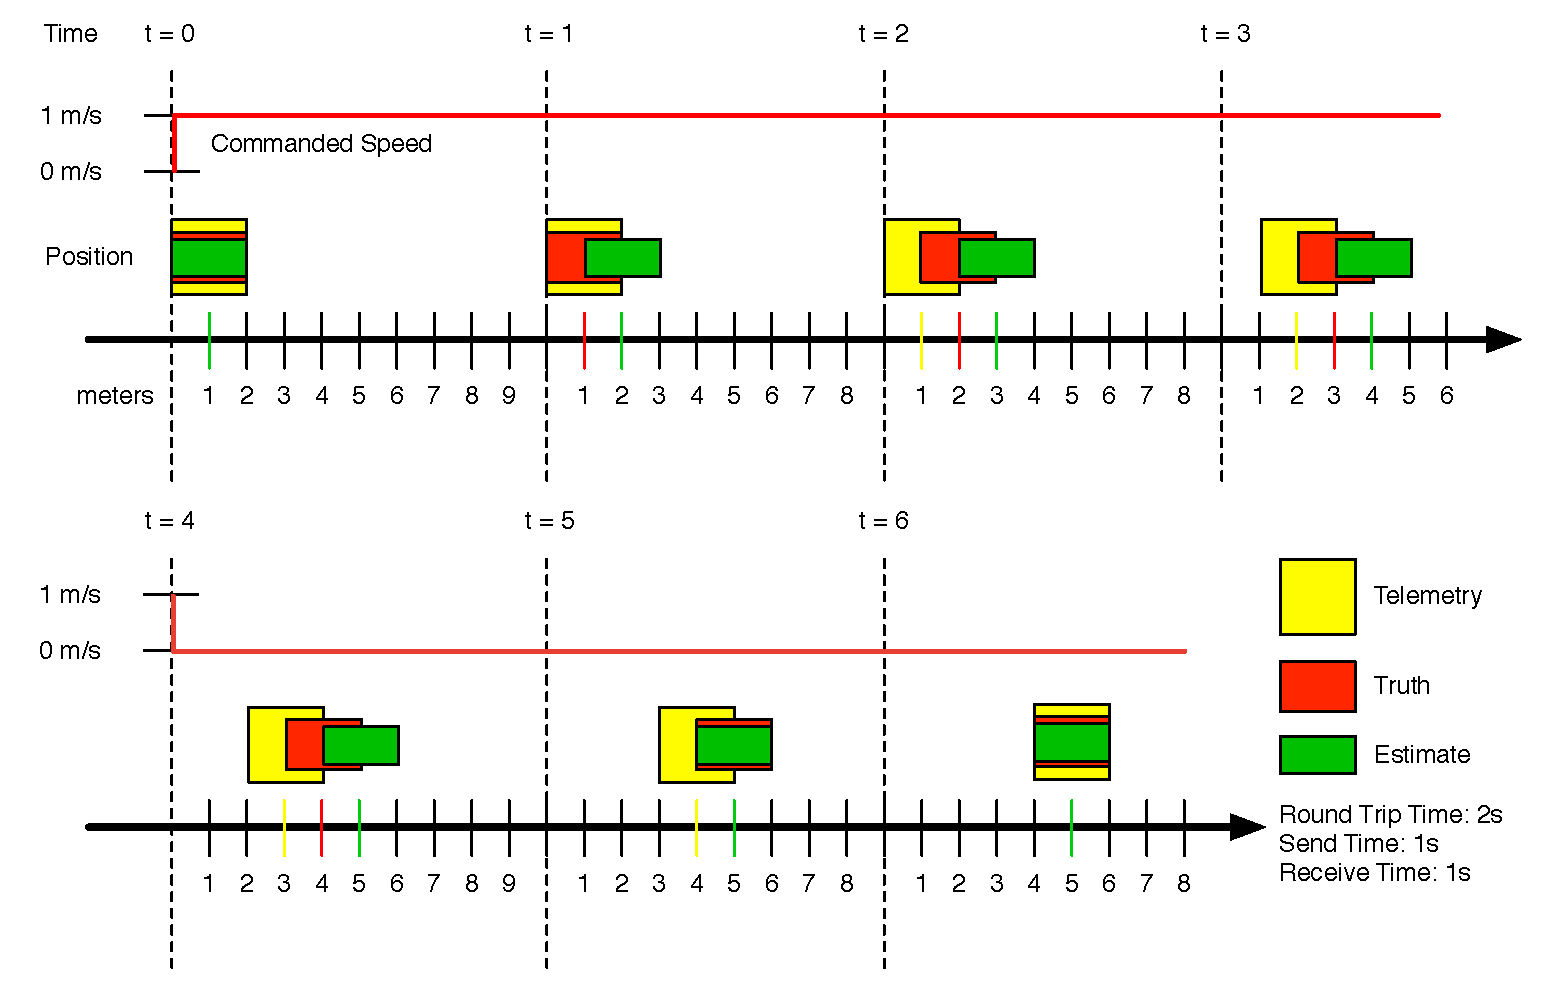
\includegraphics[width=6.5in,keepaspectratio]{latency_reduction_timing.pdf}
  \caption{Shows the limit of the estimate, in this figure the RTT latency is two seconds, one second in both directions}
  \label{fig:latency_reduction_timing}
\end{figure}

Figure \ref{fig:latency_reduction_timing} shows process of the estimation with a vehicle starting at stand still and driving forward for a brief time.  In the figure the RTT is two seconds which means that there is one second before commands reach the robotic vehicle, and an additional second before telemetry of the movement is received by the teleoperator computer.  The figure shows that the estimate moves immediately with input from the teleoperator, but since it takes one second for the robotic vehicle to receive the command, the truth data does not move one meter until two seconds into the scenario.  Finally, three seconds into the scenario the teleoperator will observe the telemetry of the robotic vehicle move one meter.  As the teleoperator decreases the commanded velocity the estimate, truth, and telemetry converge.  At a given speed the simulated vehicle position will never extend further than the speed times the RTT.

\section{Vehicle Model}
In order to produce the estimated vehicle position based on the teleoperator input, a two dimensional kinematic model of the vehicle is used to simulate the changes in position over time in this thesis.  The purpose of this thesis is to show that using a model to predict the position of the vehicle is useful for improving teleoperation performance, and the vehicle used to test is well described using a simple kinematic model.  This thesis work is designed such that a more sofisticated, dynamic model can easily be substituted is desired.  The kinematic model of the differential, non-holonomic system is given by Equation (\ref{eq:kinematic_model}).

\begin{equation} \label{eq:kinematic_model}
\zeta \; =\; \left[ \begin{array}{c} \Delta x \\ \Delta y \\ \Delta \psi \end{array} \right]\; =\; \left[ \begin{array}{c} V_{l}\; \cdot \; \Delta t \\ 0 \\ V_{\psi }\; \cdot \; \Delta t \end{array} \right]
\end{equation}

In Equation (\ref{eq:kinematic_model}) $\zeta$ is a vector that represents the change in position in the robot, or vehicle, frame.  The $\zeta$ vector has components $\Delta x$ which is displacement in $x$ direction of the robot frame, $\Delta y$ which is the displacement in the $y$ direction, and $\Delta \psi$ which is the change in heading in the robot frame.  These displacements are given by the right most vector in Equation (\ref{eq:kinematic_model}).  The $V_{l}$ term is the linear velocity from the teleoperator input, the $V_{\psi}$ is the angular velocity from the teleoperator input, and the $\Delta t$ component is the change in time between simulation steps.  The simulation is stepped by a constant $\Delta t$ so a estimated path is produced, not just a estimate for the current position or for each change in teleoperator input.

For each set of changes in the position, $\zeta$, the changes must be rotated into the odometry frame from the robot frame.  This rotation is given by the rotation matrix in Equation (\ref{eq:2d_rotation}).

\begin{equation} \label{eq:2d_rotation}
R \; =\; \left[ \begin{array}{ccc} \cos \; \psi  & -\sin \; \psi  & 0 \\ \sin \; \psi  & \cos \; \psi  & 0 \\ 0 & 0 & 1 \end{array} \right]
\end{equation}

In Equation (\ref{eq:2d_rotation}) the $\psi$ term is the current vehicle heading.  This rotation matrix is multiplied by the $\zeta$ vector in Equation (\ref{eq:kinematic_model}) to rotate those changes into the odometry frame, and then these changes in the odometry frame are added to the existing robot state, completing the simulation step.  This is shown in Equation (\ref{eq:update_kinematic}).

\begin{equation} \label{eq:update_kinematic}
\left[ \begin{array}{c} x \\ y \\ \psi  \end{array} \right]\; =\; \left[ \begin{array}{c} x \\ y \\ \psi  \end{array} \right]\; +\; \left( R\; \cdot \; \zeta  \right)
\end{equation}

The simulation is iterated as described until the simulation time matches the current time.  The result is a series of states from the time of the latest robotic vehicle telemetry to the current time.  In order to use this data to assist the teleoperator the data must be visualized in a useful manner, which is discussed in the following section.

\section{Visualizing the Estimate}
Like the visualization of the mapping system, which is described in the Section \ref{sec:rendering_the_map}, the visualization of the model prediction is done in rviz.  Initially each of the simulation states were inserted into a `Path' message, which is a list of positions which are rendered as a line.  This gave the teleoperation an arc, which originated from the telemetry origin, and indicated the path the vehicle would take.  This method had a draw back, in that when the robotic vehicle was commanded to turn in place, no line was given, as the simulated states all have the same position, but different headings.

To solve the issue of zero radius turning, an array of arrows were used, instead of a line, to display the predicted path of the vehicle.  This method allowed for indication of motion when turning in place while still providing a good indication of the path when driving straight and turning.  One problem with just using the array of arrows is that when the telemetry from the robot is being displayed using a three dimensional model of the robot, the arrows tend to get covered up.

To further help the teleoperator make use of the model predictions a duplicate three dimensional model of the robot is placed at the current estimated position.  This model is colored red and gives an indication of the position of the robot as the teleoperator varies their input.  Figure \ref{fig:latency_ss} shows the red three dimensional model leading the light colored telemetry model of the robot, indicating the position of the vehicle due the input from the teleoperator.  The image on the right in Figure \ref{fig:latency_ss} shows the model prediction from below the vehicle, which reveals the array of arrows representing the path being taken by the model prediction.  These arrows are normally hidden to the teleoperator, but the teleoperator could rotate the camera to see them if they wish.

\begin{figure}[ht]
  \centering
  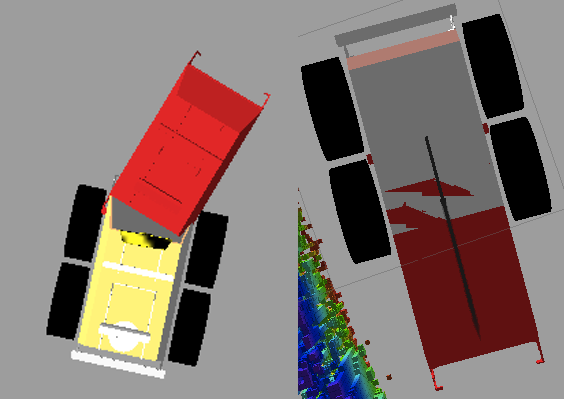
\includegraphics[width=5in,keepaspectratio]{latency_ss.png}
  \caption{Example of the model prediction visualization, the left image is a top down view, and the right image is a bottom up view}
  \label{fig:latency_ss}
\end{figure}

Experiments designed to test the effect of the vehicle model prediction in the presence of latency are described in Section \ref{sec:latency_reduction_trials}.

%%%%%%%%%%%%%%%%%%%%%%%%%%%%%%%%%%%%%%%
%% Chapter: Experiments
%%%%%%%%%%%%%%%%%%%%%%%%%%%%%%%%%%%%%%%

\chapter{Latency Reduction and Three Dimensional Mapping Experiments}\label{chap:experiments}
This chapter covers the latency reduction and three dimensional mapping experiments, the hardware and software systems used execute the experiments, and the results of the experiments.  The goals of the experiments are outlined, showing their purpose and relevance.  In order to carry out the described experiments a experimental test fixture was constructed, consisting of various hardware and software components, which are described in detail here due to their bearing on experiment setups.  The experimental methodology is also described here, which points out the elements that influence the results of the experiments.

\section{The Experimental Test Fixture}\label{sec:robotic_vehicle}
To facilitate the latency reduction experiments and the three dimensional mapping experiments several robotic test vehicles were constructed.  All of the robotic vehicles had some similar components and used similar navigation techniques and software.  Each robotic vehicle was equipped with a Sick LMS151 LiDAR which provided two dimensional data about the environment and wheel encoders which were integrated over time to provide odometry measurements.  Additionally, each vehicle combined the LiDAR data with the wheel odometry using SLAM\cite{grisetti2007improved}\cite{grisettiyz2005improving} to provide an accurate indoor navigation solution.  Though configurations for the wheel odometry and SLAM algorithm differed between vehicles, each vehicle used similar setups to provide accurate two dimensional poses of the robot indoors.

Each vehicle also provides three dimensional data about the environment using one of the RGB-D camera systems available, like the Microsoft Kinect or the ASUS Xtion Live Pro.  Early experiments and data sets used the Microsoft Kinect as the three dimensional data source, but the final system tests used the ASUS Xtion Pro Live.  This due to the ASUS Xtion Pro Live hardware image registration and simpler power requirements.  One other advantage to the ASUS Xtion Pro Live is that it is smaller, lighter, and easier to mount that the Kinect, which made adjusting and calibrating the sensor much simpler.

\subsection{SegwayRMP 200}
Though there are many similarities in the different robotic vehicle test fixtures, the hardware configuration of each differed significantly.  There have been three robotic vehicle platforms during the course of this research.  The first system was based on a Segway RMP200 ATV platform.  This robotic vehicle had a Mac Mini with a 2.6GHz Core 2 Duo processor and four gigabytes of RAM.  The sensor package consisted of a Sick LMS151, wheel odometry, and a Microsoft Kinect.  This platform was electrically damaged a few months into the research and new platform had to be pursued.  Only a small amount of data collected with machine was used in the final research, but it served as a learning platform when the first proof of concepts for this work were underway.  Additionally, a software artifact in the form of the library `libsegwayrmp' resulted from this part of the work.  The library is middleware agnostic, i.e. not ROS or MOOS specific, and is in use at as many as ten different institutes outside of Auburn to date.  The hardware configuration of the Segway RMP200 vehicle can be seen in Figure \ref{fig:segway_rmp200}.

\begin{figure}[ht]
  \centering
  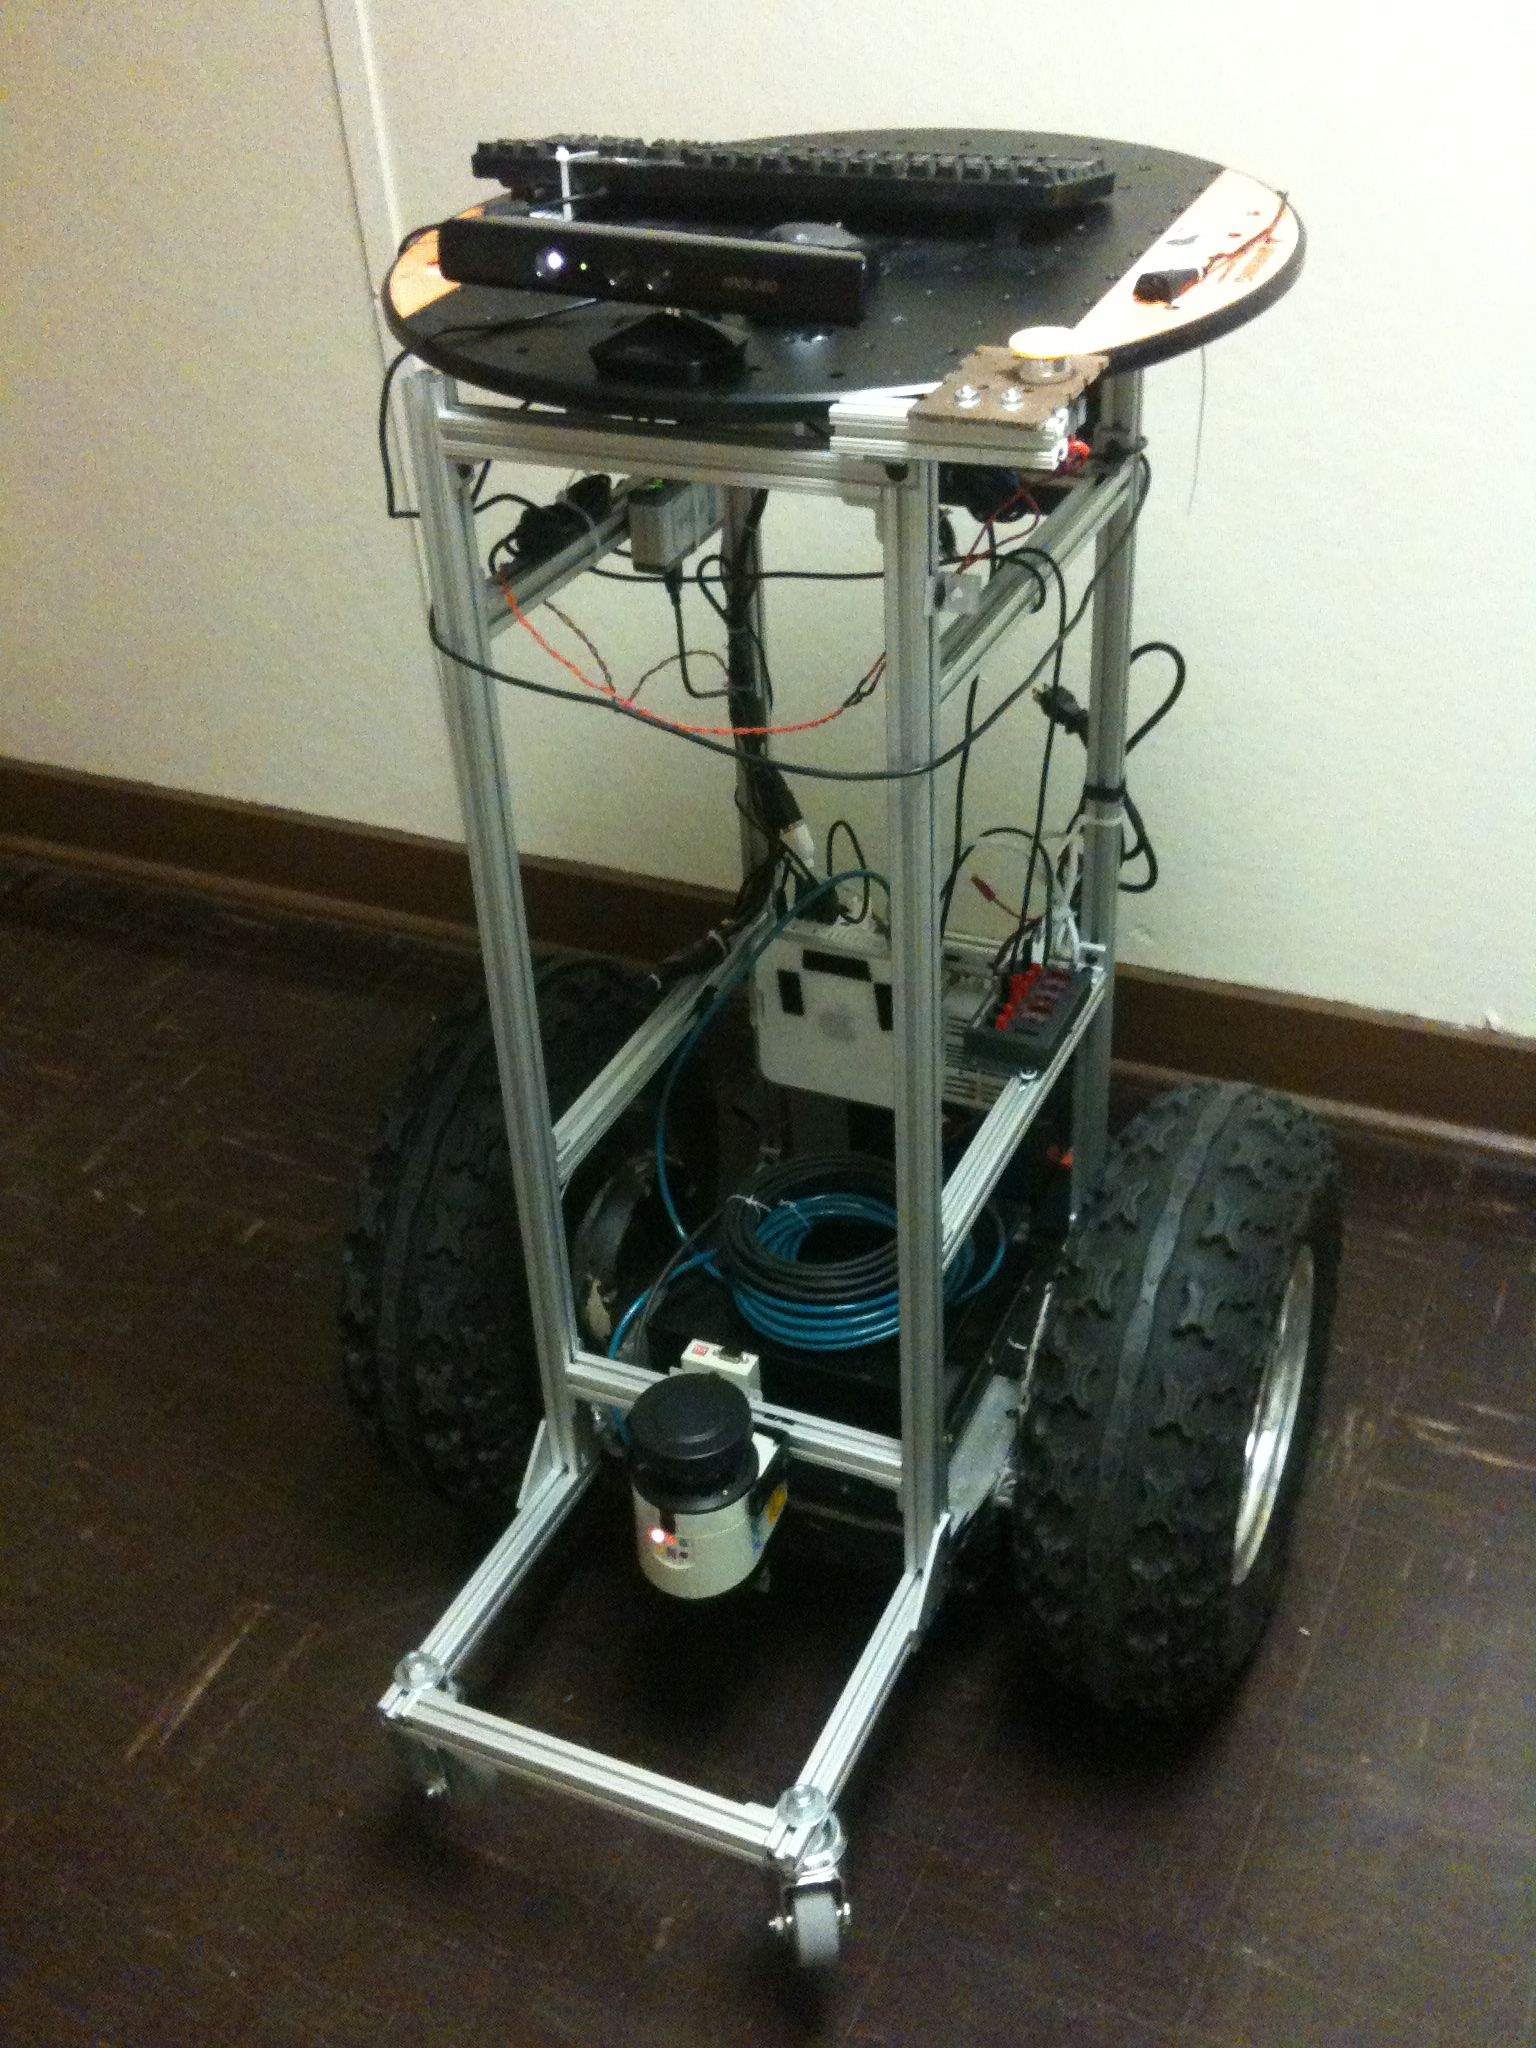
\includegraphics[width=4in,keepaspectratio]{segway.jpg}
  \caption{Segway RMP200 ATV Robotic Vehicle Platform}
  \label{fig:segway_rmp200}
\end{figure}

\subsection{Autonomous Lawnmower}
The second robotic vehicle used as the test fixture was to be an iRobot ATRV, but this vehicle needed a lot of work before it would be useful for research.  In the mean time, to collect data for a publication, the Auburn autonomous lawnmower was used as a robotic vehicle platform for a short time.  Data taken on the autonomous lawnmower was used in this thesis work and was used in another publication related to this work.  Like the Segway platform, the lawnmower has the Sick LMS151, the Microsoft Kinect, and wheel odometry.  Additionally, it has the Point Grey Research Bumblebee2 stereo vision system which produces three dimensional data similar to the data produced by RGB-D sensors.  The lawnmower has less accurate odometry, due to low resolution encoders, and this increased the error discussed in the Section \ref{sec:uncertainty}.  The autonomous lawnmower and its hardware configuration for this thesis work can be seen in Figure \ref{fig:lawnmower}.

\begin{figure}[ht]
  \centering
  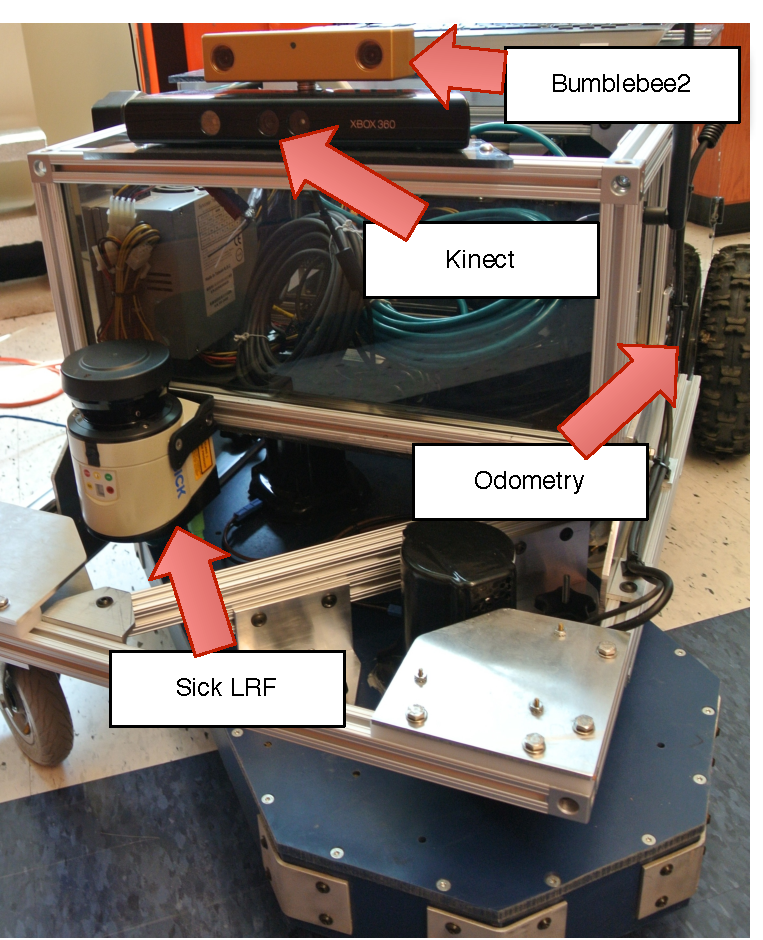
\includegraphics[width=4in,keepaspectratio]{lawnmower.pdf}
  \caption{Autonomous Lawnmower Mower Robotic Vehicle Platform}
  \label{fig:lawnmower}
\end{figure}

\subsection{iRobot ATRV}
The final robotic vehicle used as the test fixture is based on an iRobot ATRV.  This robotic vehicle is used in the latency reduction trials and is to be the basis for future work.  The ATRV is equipped with the Sick LMS151, high resolution wheel encoders, the Microsoft Kinect and the ASUS Xtion Pro Live.  The higher resolution encoders provided a much better pose estimate between SLAM updates, resulting in much better results during mapping.  The option of using the ASUS Xtion Pro Live also allowed more flexibility on adjusting the mounting and less processing while registering the color image to the three dimensional data.  The ATRV and its configuration for the latency reduction trials can be seen in Figure \ref{fig:atrv}.

\begin{figure}[ht]
  \centering
  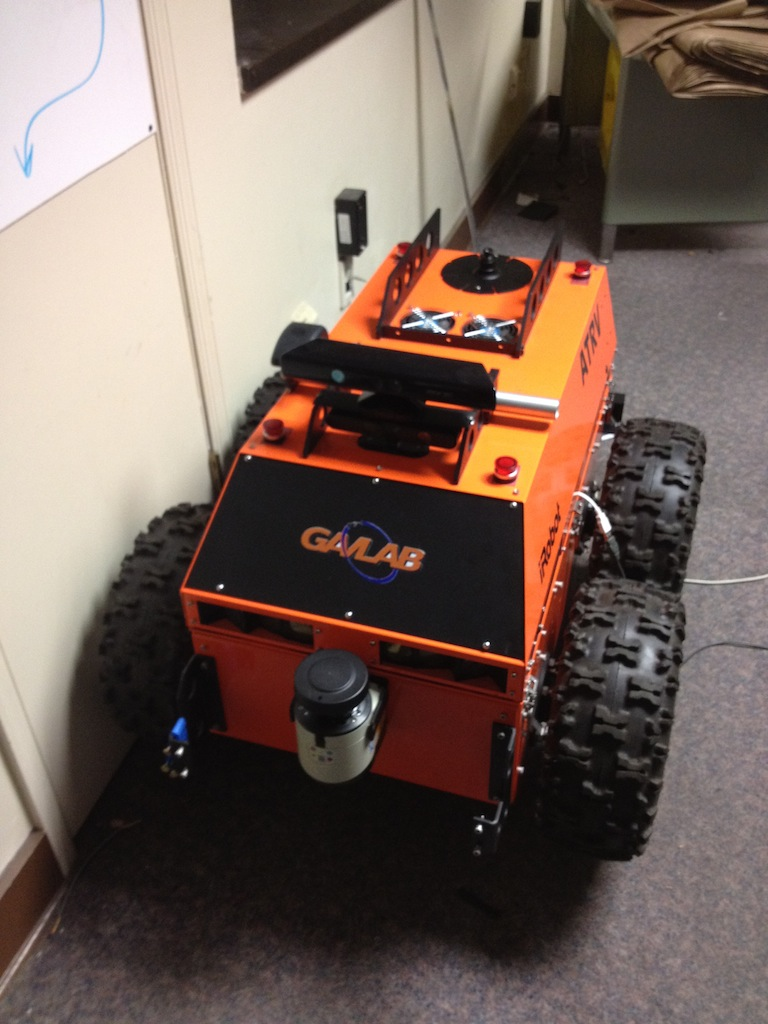
\includegraphics[width=4in,keepaspectratio]{atrv.jpeg}
  \caption{ATRV Robotic Vehicle Platform}
  \label{fig:atrv}
\end{figure}

\subsection{Software}
In addition to the robotic vehicle hardware and device interface software, there exists several software components and artifacts which were created to allow the test fixture to perform the planned experiments.  All of the robotic platforms used very similar software.  The middleware used on all of the robotic platforms was ROS, the Robotics Operating System\cite{quigley2009ros}.  ROS provides a build system, code organization tools, inter process communication, standard data types common in robotics, debugging tools, visualization tools, implementations of common algorithms, and a large open community.  Because of the common ground provided by ROS and its tools, many software packages were available to speed up the development of the robotic platforms.  For example, the ROS community provides drivers for common hardware, some of which was used on the test fixtures.  ROS provides an complete and efficient interface to RGB-D sensors like the Microsoft Kinect and ASUS Xtion Pro Live.  Additionally, the message passing conventions and tools provided by ROS makes it very easy to abstract components of the system in a manner described in Chapter \ref{chap:system_design}.  Because of the well defined interfaces and decoupling of the software components, the mapping system can use data from either the ASUS Xtion Pro Live or the Microsoft Kinect with absolutely no changes to the source code.  With drivers for the RGB-D sensors and tight integration with perception libraries like octomap and PCL, ROS was the best engineering decision for the robotic platform and this work.

Working with ROS involves several software tasks like wrapping drivers in ROS code, describing the robot's geometry in the Unified Robot Description Format (URDF), and drawing a model of the robot in blender for use in the teleoperation visualization, as shown in Figure \ref{fig:atrv_blender}.

\begin{figure}[ht]
  \centering
  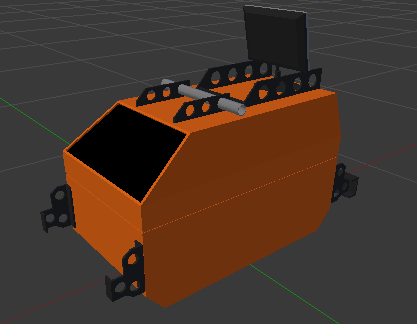
\includegraphics[width=4in,keepaspectratio]{atrv_blender.png}
  \caption{ATRV Robotic Vehicle Platform in Blender}
  \label{fig:atrv_blender}
\end{figure}

The approach for writing hardware interfacing software, or drivers, and other programs in ROS is to make an agnostic library with a thin layer of ROS specific code around it, often called a wrapper.  This design pattern allows the majority of the code to remain agnostic of the middleware, allowing software to move to another middleware or to a monolithic system on a micro-controller or in a product, if needed.  The geometry of the robot is described in a generic format called the URDF.  Once the robot was setup with a URDF and all of the hardware interfaces were working, the vehicle was ready to have its sensors visualized and recorded.  Using rviz, the sensors on the vehicle can be visualize because they all adhere to the common data types defined by the ROS community.  

In addition to the message passing between programs and data visualization, the logging system needed to be able to keep up with the Kinect and laser data.  The Kinect, and similar sensors, produce significant amounts of data and the logging system would need to be very efficient in order to keep up with the high data rates.  Table \ref{tab:kinect_data} shows how much data is produces by the Kinect at different resolutions.

\begin{table}[h]
\caption{Bandwidth of Raw Kinect Data at Different Resolutions}
\label{tab:kinect_data}
\begin{center}
  \begin{tabular}{ | l | c | c | }
    \hline
    ~ & Resolution & Megabytes per second \\
    \hline
    VGA & 640x480 & 76.6 \\
    QVGA & 320x240 & 50.5 \\
    QQVGA & 160x120 & 30.5 \\
    \hline
  \end{tabular}
\end{center}
\end{table}

The rates in \ref{tab:kinect_data} are empirical because the actual rate can be effected by the scene being imaged.  The number of points converted from the depth map can change due to the effects of some scene configurations, for example where a close object shadows other objects in the room obstructing them from the point cloud data.  The data rate can fall from the maximum thirty hertz if the system is over taxed or if data is purposely dropped to reduce processing costs.  Even with these reductions in the amount of information, recording all of the sensors on the robotic vehicle system results in log files that are two to four gigabytes per minute in size.

These software components together enable a test fixture that can reliably execute commands and collect data for the three dimensional mapping and latency reduction trials.  Having a stable and well designed test fixture and test implementations are a crucial component to enabling this research to move forward.

\begin{figure}[ht]
  \centering
  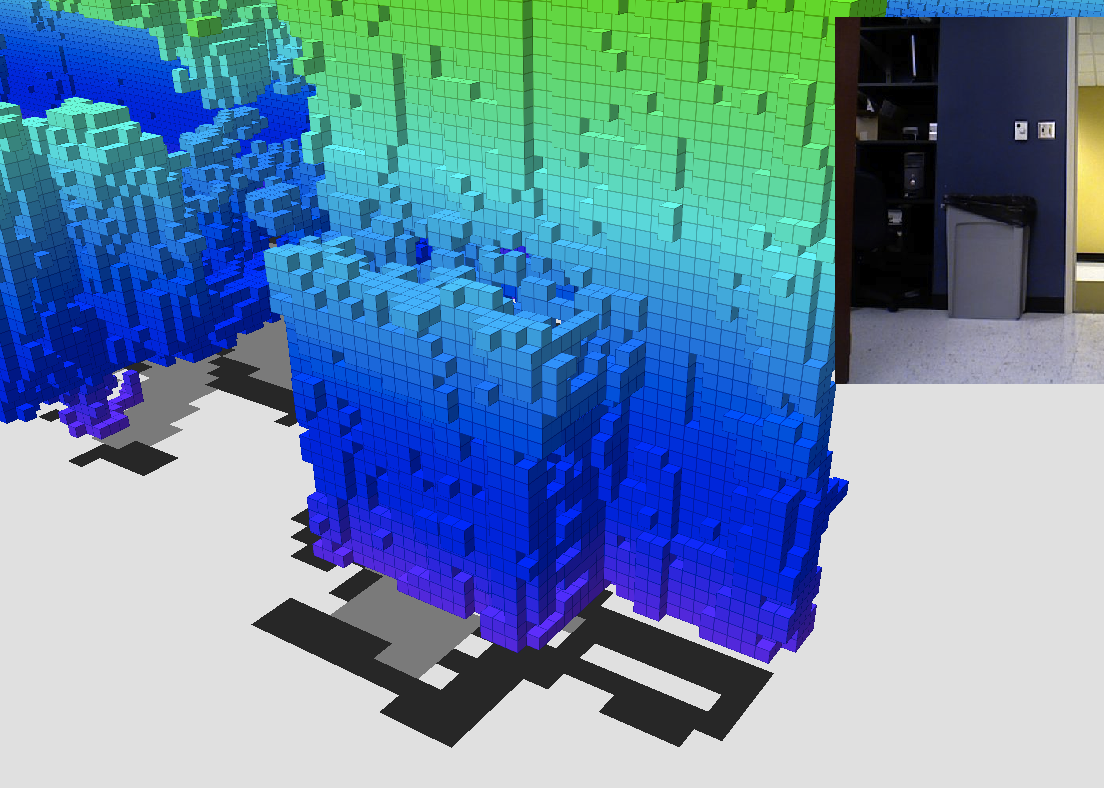
\includegraphics[width=6.5in,keepaspectratio]{mapping_trashcan.png}
  \caption{Results from one of the three dimensional mapping acceptance tests, with the three dimensional map above the SLAM map(left), and an image of the scene from a color camera(right)}
  \label{fig:mapping_trashcan}
\end{figure}

\section{Three Dimensional Mapping Experiments}
The experiments, which are responsible for validating the three dimensional mapping system, take the form of acceptance tests.  Acceptance testing is simply running the software manually over a give set of inputs and manually examining the results.  Due to the fact that mapping system can be run off recorded data sets, i.e. there is no closed loop from the teleoperator, the mapping system can also be tested against recorded data sets.  Using the flexibility of recorded data sets, a series of acceptance tests were devised using select data sets which were known to cause problems or errors in the mapping process.  These acceptance tests are executed by simply running the mapping system over each of the previously selected data sets and visually examining the results.  The results can be affected by changes in the mapping system or by changes in the navigation system of the robot.  Therefore data contained in the test data sets contain all of the data needed to recompute the navigation solution off-line.  Recomputing the navigation solution with different parameters allowed the mapping system to be tested under different noise and error conditions without rerunning the robot under different settings.  Figure \ref{fig:mapping_trashcan} shows the results from one of the three dimensional mapping acceptance tests, with the three dimensional map above the SLAM map on the left, and an image of the scene from a color camera on the right.

In addition to testing the three dimensional mapping portion of the overall system, these acceptance tests provide an opportunity to test parts of the teleoperation system like the transmission of the maps between computers.  Figure \ref{fig:map_bandwidth} shows some statistics about the bandwidth required to transmit the map over the network during one of the test data sets.

\begin{figure}[ht]
  \centering
  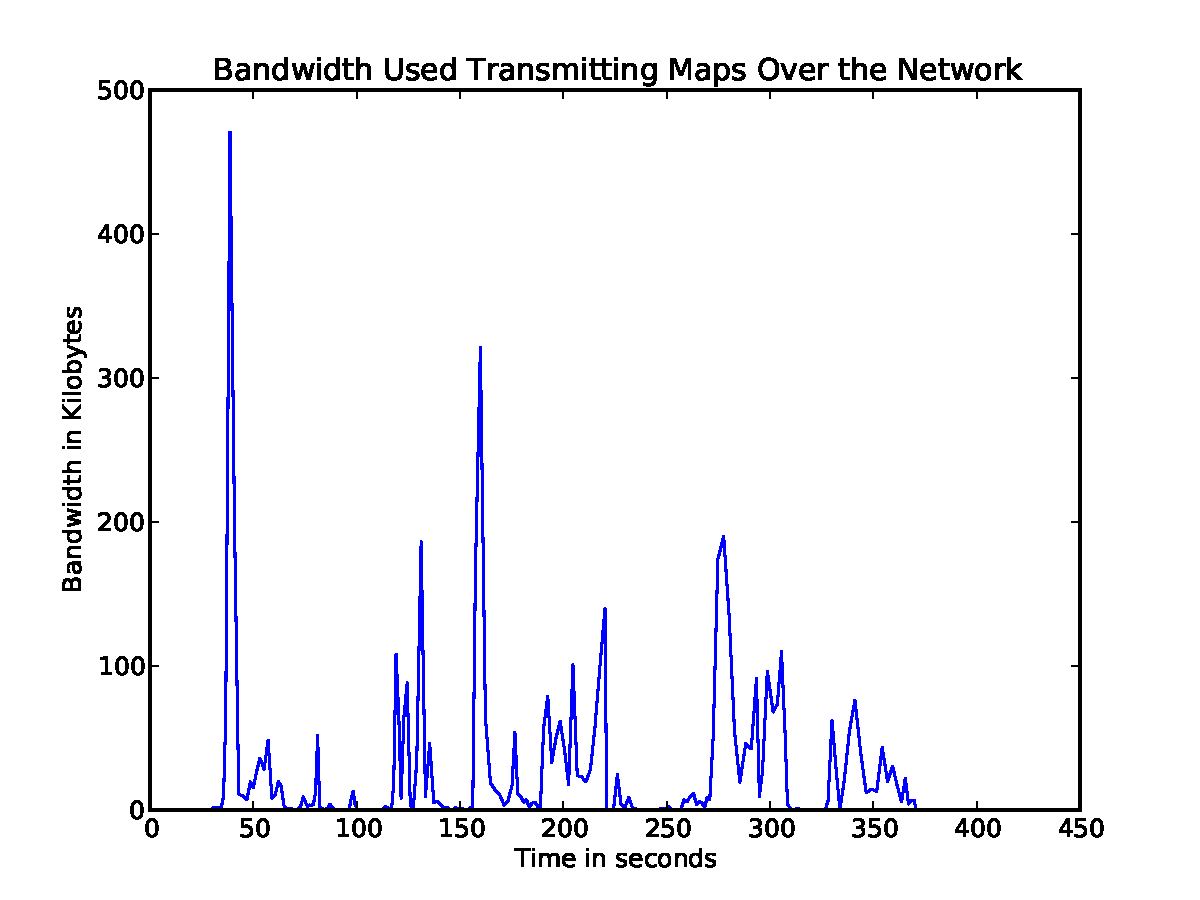
\includegraphics[width=6.5in,keepaspectratio]{map_bandwidth.pdf}
  \caption{Bandwidth usage for transmitting the map over the network versus time}
  \label{fig:map_bandwidth}
\end{figure}

In Figure \ref{fig:map_bandwidth} the bandwidth limit was set to infinity, setting no constraint on the bandwidth usage over a period of time.  If a bandwidth constraint were to be placed on the synchronization system, then when the amount of data being sent divided by the synchronization period is greater than the constraint limit, a down-sampled version of the map differences would be sent.  This down-sampling action is made very efficient because of the nature of octrees.  Because the down-sample changes are united with both the client map on the teleoperator computer and the vehicle computer subsequent iterations of the synchronization process will send the high resolution differences at a later date.  Looking at the data in Figure \ref{fig:map_bandwidth}, the large peaks correspond with periods when the vehicle is mapping new areas.  When new areas are being mapped for the first time the map must be expanded and a lot of newly occupied cells are transmitted in the changes.  Conversely, when the vehicle is traveling though areas it has been before the amount of bandwidth consumed is reduced resulting in periods of low bandwidth usage.

\section{Latency Reduction Trials}\label{sec:latency_reduction_trials}
In order to measure the effectiveness of the latency reduction techniques described in Chapter \ref{chap:latency_reduction}, a series of trials are performed and recorded.  The purpose of these trials is to show the effect of latency on the teleoperators, and the improvement of teleoperation when using the three dimensional map and a predictive vehicle model.  These trials involved driving the vehicle under varying teleoperation setups with varying latencies induced on the system.  A test course was setup in and around the lab to try and have a repeatable, short, and challenging environment to test the teleoperators against.  Figure \ref{fig:latency_reduction_map} shows the path the vehicle takes during the trials.

\begin{figure}[ht]
  \centering
  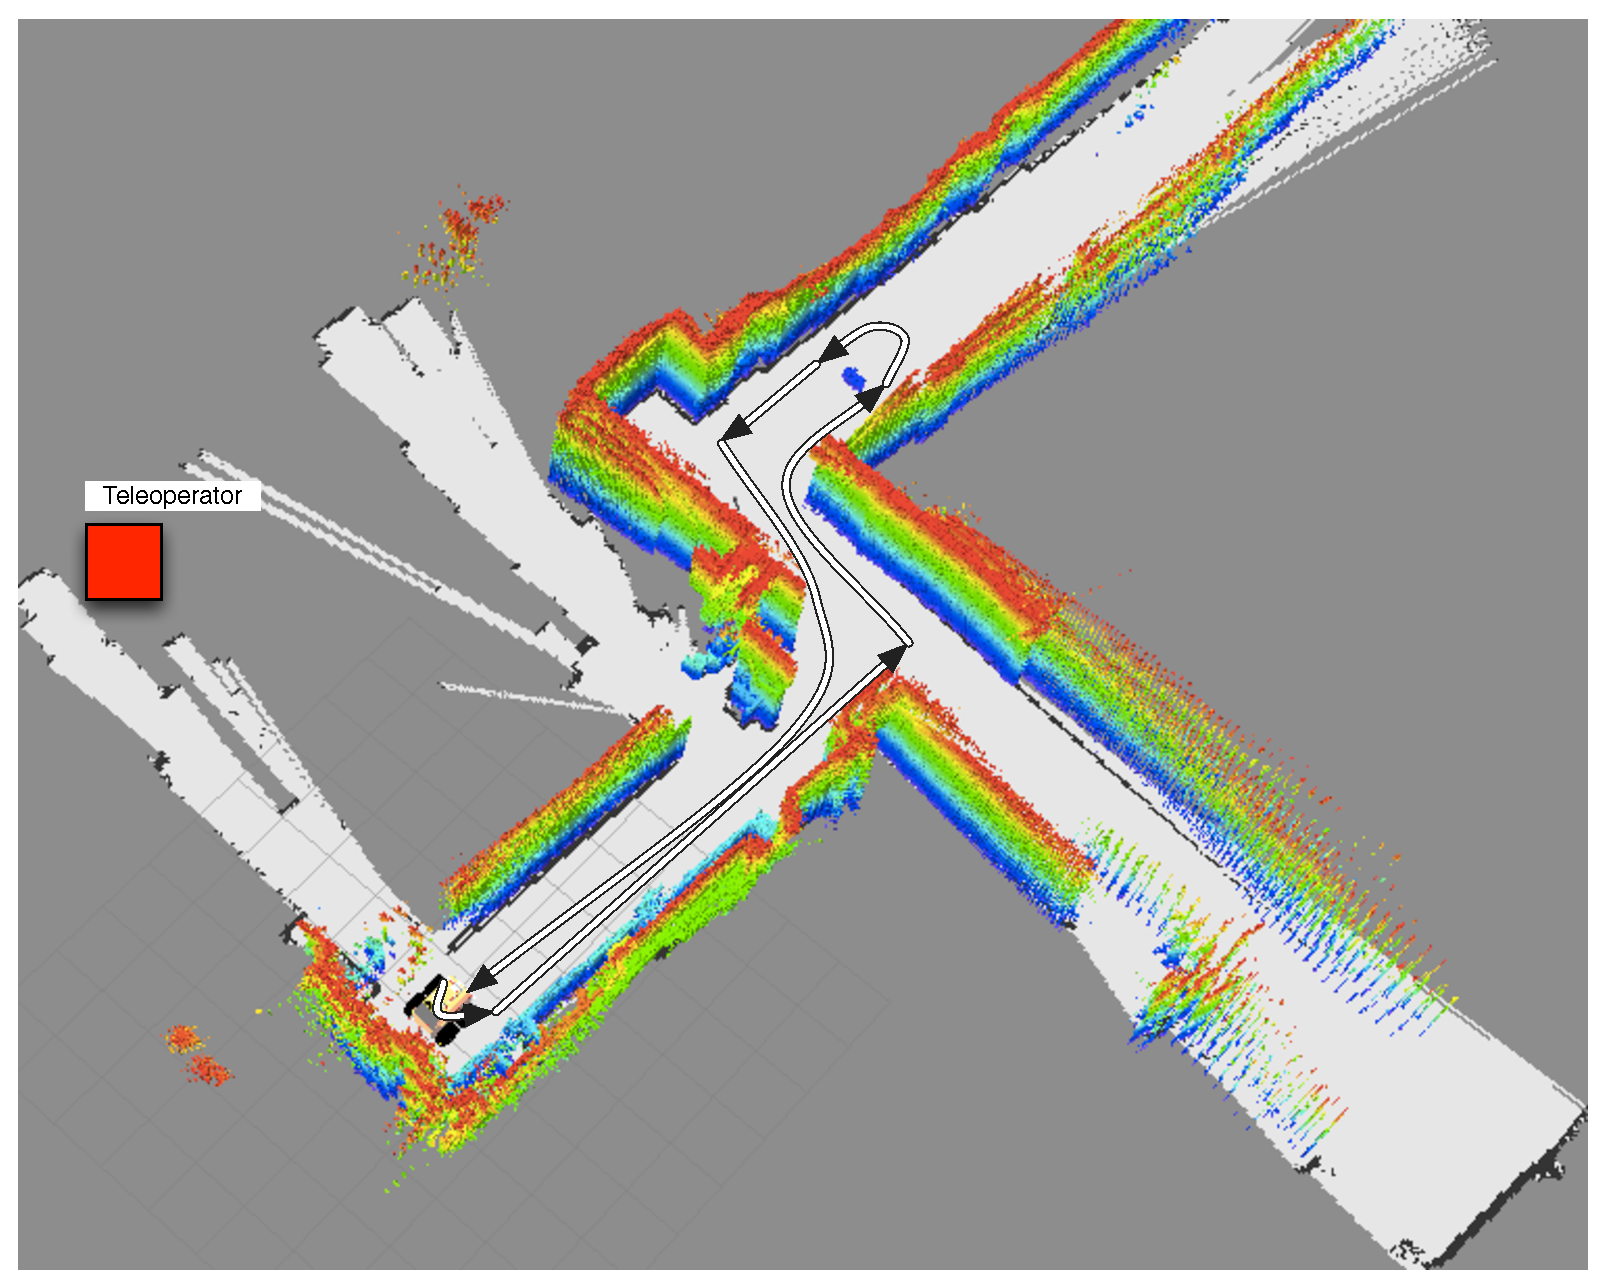
\includegraphics[width=6.5in,keepaspectratio]{latency_reduction_map.pdf}
  \caption{Map of the path taken by the robotic vehicle during the latency reduction trials}
  \label{fig:latency_reduction_map}
\end{figure}

The vehicle begins in the lab, at its charging station, where it can be seen in the bottom left corner of Figure \ref{fig:latency_reduction_map}.  The teleoperator must rotate the vehicle and drive the length of the lab and exit through the door into the hallway.  In the raw trial data in Appendix \ref{chap:latency_results} that stretch of the course is referred to as `Segment 1'.  `Segment 2' is the vehicle traveling from the door frame to the obstacle in the hallway, seen at the top of the path in Figure \ref{fig:latency_reduction_map}.  `Segment 3' is part of the course where the vehicle is maneuvering around the obstacle and ends when the vehicle has cleared the left side of the obstacle and is returning to the door.  The final segment, `Segment 4' is the vehicle traveling from the obstacle in the hall back through the door of the lab.  Finally the total time is marked when the vehicle is back where it started next to the charging station in the lab.  In addition to travel times the number of hits or potential hits of the vehicle are recorded.  A hit is counted as any time the vehicle touches an obstacle or wall along the course.  Additionally, the safety person following the vehicle while it is traversing the course will notify the teleoperator if they about to strike something, which is also counted as a strike.  Figure \ref{fig:latency_reduction_map} also shows the location of the teleoperator during the trials.  The position of the teleoperator prevents them from having visual contact with the vehicle at any point during the trial.  The teleoperator is using a workstation which is running the teleoperation visualization software and that is equipped with a gamepad for driving the vehicle.  

For each run of the trials, the conditions are different.  There are three different latency settings and three different teleoperation setups used in the trials.  The three teleoperation setups are: front facing camera only, camera and three dimensional map, and camera, three dimensional map, and predictive vehicle model.  For each teleoperation setup three different latencies are used: no latency, one second round trip time, and two second round trip time.  This totals to nine permutations for the trials, but since running the predictive vehicle model with no latency has no effect that particular permutation is ignored, resulting in eight total runs by each teleoperator.  To try and curb any learning bias or progression bias, the teleoperators are given the different scenarios in random order.  Before the trials begin the teleoperators are given a test loop around the test course so that they can become familiar with the teleoperation system and the controls of vehicle.  Additionally, the three dimensional map is reset for each consecutive run.

It should be noted that the teleoperator, in the case of three dimensional map and three dimensional map with predictive vehicle model, only had access to the three dimensional map and the position of the vehicle.  Figure \ref{fig:latency_reduction_map} shows the three dimensional map and the SLAM map, which is not available to the teleoperators, because it is a by product of the navigation solution.  On an outdoor vehicle, the SLAM map may not be available, therefore it was excluded from the data presented to the teleoperator.

\begin{figure}[ht]
  \centering
  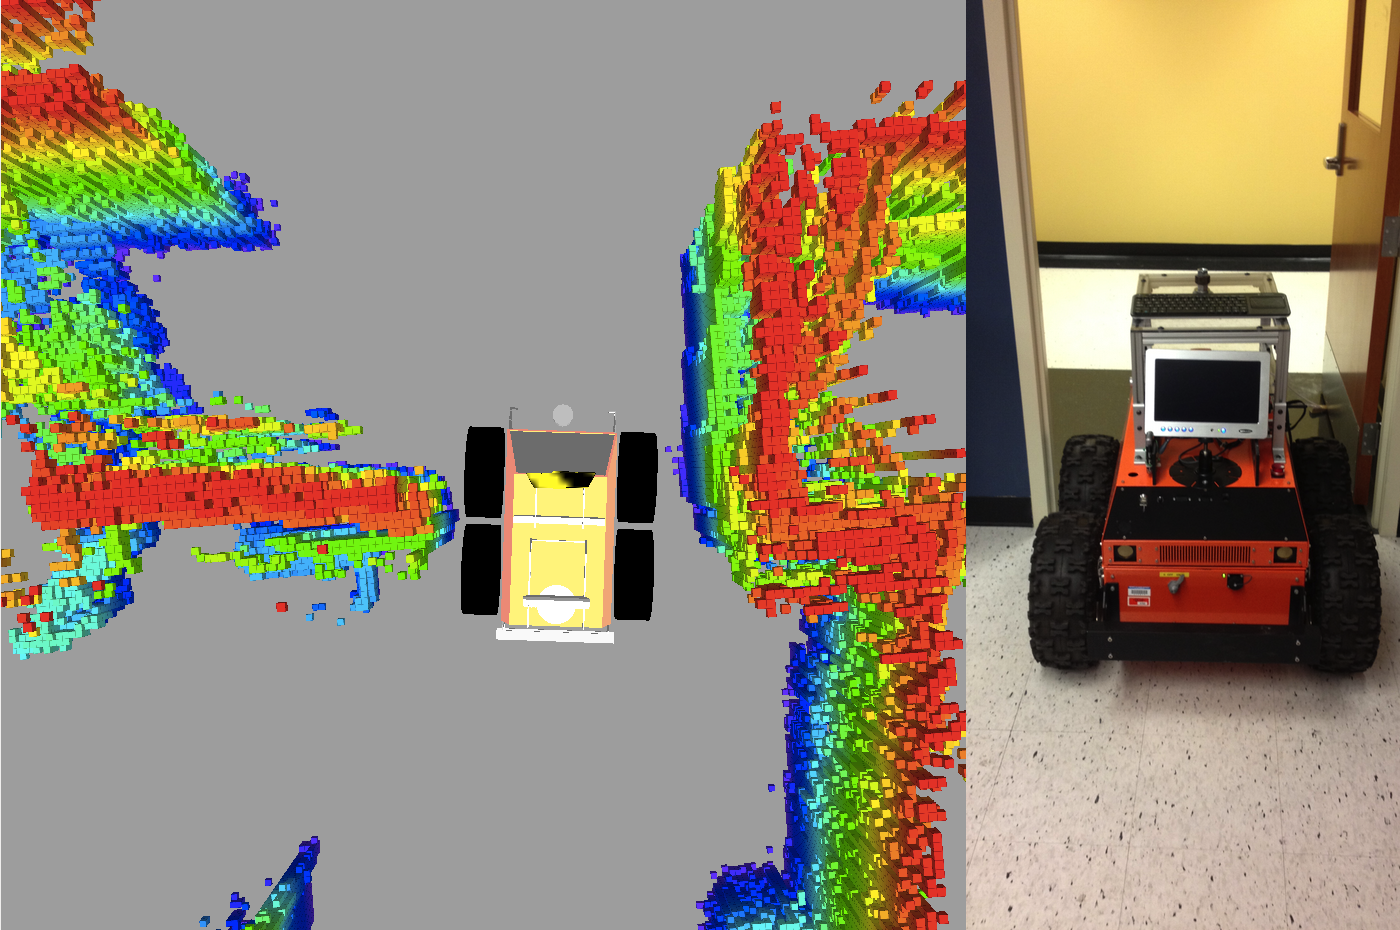
\includegraphics[width=6.5in,keepaspectratio]{3d_map_doorway.png}
  \caption{Top down view of the robotic vehicle navigating through a doorway using the three dimensional map as a reference(right), and a camera picture from behind during the navigation through the doorway(left)}
  \label{fig:3d_map_doorway}
\end{figure}

Figure \ref{fig:3d_map_doorway} shows a more typical view for the teleoperator on the left and a camera picture of the vehicle passing through the same doorway on the right.  The setup on the left is the three dimensional map only, no predictive vehicle model, but is properly lacking the two dimensional SLAM map as described above.

The complete results of the latency reduction trials are listed in Appendix 1.  Figure \ref{fig:trial_times} shows the average times for each of the trial scenarios.

\begin{figure}[ht]
  \centering
  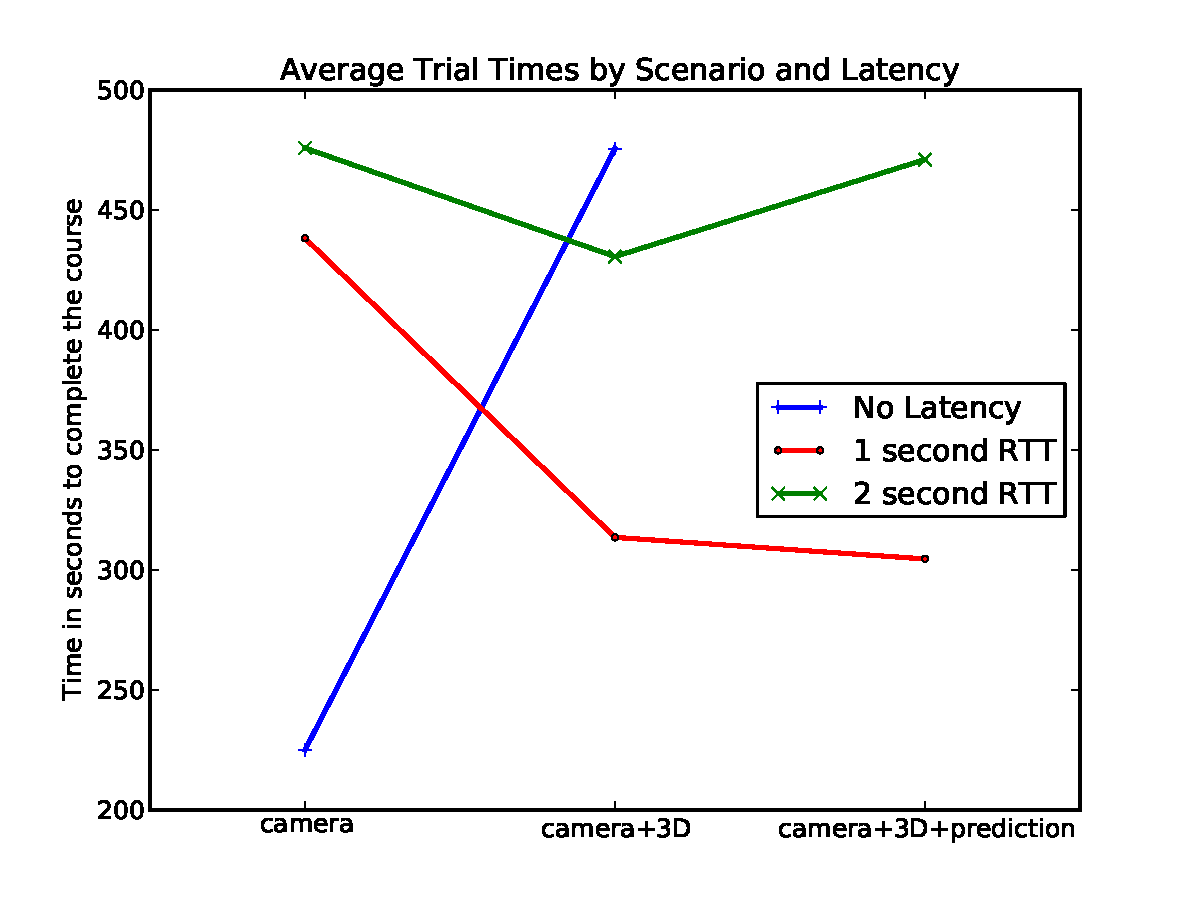
\includegraphics[width=6.5in,keepaspectratio]{trial_times.pdf}
  \caption{Average time to complete the trial course in seconds by scenario and latency}
  \label{fig:trial_times}
\end{figure}

Figure \ref{fig:trial_hits} shows the average number of hits, actual and near hits that were prevented, plotted against each teleoperation scenario and for each latency setting.

\begin{figure}[ht]
  \centering
  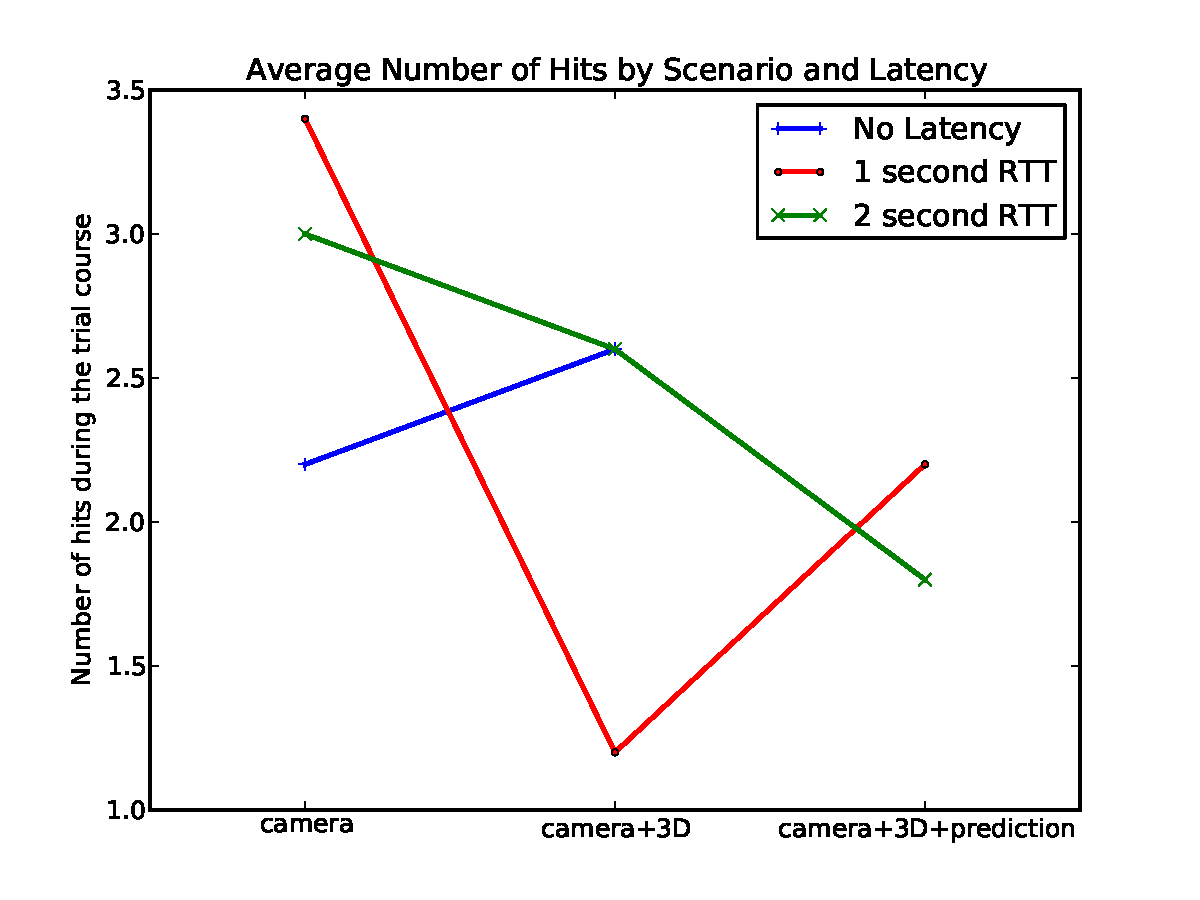
\includegraphics[width=6.5in,keepaspectratio]{trial_hits.pdf}
  \caption{Average number of hits during a trial run by scenario and latency}
  \label{fig:trial_hits}
\end{figure}

Figures \ref{fig:trial_times} and \ref{fig:trial_hits} are averages over the five sets of results from the trials, but the individual teleoperators varied considerably. as some teleoperators were cautious and others were aggressive, causing different ratios of times to hits for each teleoperator.  In addition to differences in style, the teleoperators differed considerably in overall skill.  Some teleoperators outperformed their peers in both time and number of hits.  Consistency in the teleoperators was also a problem, where some results departed from what was common place due to getting stuck at a particular part or by getting lucky with avoiding an obstacle.  All of these problems and the problem of teleoperators improving through learning can be diminished with larger sample sizes.

%%%%%%%%%%%%%%%%%%%%%%%%%%%%%%%%%%%%%%%
%% Chapter: Conclusions
%%%%%%%%%%%%%%%%%%%%%%%%%%%%%%%%%%%%%%%

\chapter{Conclusion}\label{chap:conclusion}
This thesis has shown that three dimensional maps of the environment can be constructed using novel three dimensional sensors like the Microsoft Kinect and ASUS Xtion Pro Live, and that applying those maps to aid in teleoperation can make improvements in teleoperation speed and accuracy.  Furthermore, this thesis work has shown that latency can cause teleoperation performance to slow down and become more error prone, and that using a vehicle model can help reduce the effects of latency.  The predictive vehicle model is especially useful in high latency systems, but would also be useful in faster moving systems with moderate latency.

From discussions with the teleoperators that performed the latency reduction trials and from the data results of the latency reduction trials some conclusions can be drawn, and other speculations made.  From the results and watching the teleoperators it is obvious that latency, especially high amounts of latency are extremely detrimental to teleoperation.  There is a relationship between the amount of tolerable latency and the speed of the vehicle.  Since the robotic test vehicle was relatively slow, about one meter per second, a larger amount of latency was tolerable.  Latencies of 500 milliseconds RTT were scarcely different from no latency on the ATRV, but if the vehicle traveled faster, say 5 meters per second, then 500 milliseconds of latency RTT might not be acceptable.

The consensus amongst the latency reduction trial teleoperators was that the thee dimensional map of the environment was most useful when navigating tight obstacles like the doorway.  With only a camera it was difficult to navigate near obstacles which had fallen out of the field of view of the camera.  For instance the doorway was difficult unless you lined up perfectly before driving through with only the camera.  With the three dimensional map the teleoperator has some notion of where the vehicle is in relation to obstacles on the sides of the vehicle or behind the vehicle.  This helps to adjust the course of the vehicle when near obstacles that are not in front of the vehicle.

A trend in the data suggests, however, that the teleoperators were faster using just the camera.  The theory here is that without additional spatial information the teleoperator has to just go through or past obstacles somewhat blindly.  When the three dimensional data is available the teleoperators are more careful when navigating obstacles, constantly adjusting the three dimensional camera to check if the vehicle is clearing the obstacles.  If there was an automatted method for selecting the best camera angle, some time could be saved.  Though the data suggests that less obstacles are hit when using the three dimensional map and predictive vehicle model, the teleoperators do not produce perfect, hit free runs even with the assistance.  Sometimes when errors in the mapping system would occur and produce incorrect maps, the teleoperators would make errors, so some of the hits during three dimensional assisted trials might be due to problems with the mapping system.

Some of the teleoperators did not find the predictive vehicle model to be consciously useful, but there seemed to be less over shooting when turning in place and the teleoperators moved forward with more confidence when they had the predictive vehicle model.  There seemed to be a subconscious improvement from the predictive vehicle model, allowing for more confident movement and longer spurts of movement as well.  Some teleoperators, however, found the predictive vehicle model very useful and preformed much better with it than without it.  Especially when turning in place and when making fast short linear movements.  Another important aspect of the predictive vehicle model is that it gives instant visual feedback to the teleoperator's input to the gamepad.  Without the immediate visual feedback, the teleoperators actions become mentally decoupled with the perceived robot movement, which is pointed out in the the work from Huber, et. al. at Carnegie Mellon University\cite{photo_real}.

The predictive vehicle model did not perfectly match the motion of the robotic vehicle in all cases.  The linear displacement of the model matched that of the vehicle fairly well, but the in place turning estimate was less accurate.  This is due, in part, to the fact that the ATRV does not perfectly execute the commanded angular velocity.  For example, when the vehicle is commanded zero linear velocity and 0.2 angular velocity, the ATRV might turn in place at 0.1 angular velocity.  This causes a discrepancy in the predicted and actual change in heading.  The heading error and other errors could be alleviated in two different fashions.  The robotic vehicle could be made to follow commanded velocities better by integrating a yaw rate observation into the closed loop controller.  Alternatively, the vehicle model could be augmented with elements that properly describe the disparity of the commanded and actual velocities.

\section{Future Work}
This thesis work shows the viability of a system that produces a three dimensional map and that the map and other latency reducing techniques can be successfully applied to the teleoperation activities.  However, the mapping process is far from perfect, the evidence of the improvement to teleoperation is incomplete, and the scope of the experiments narrow, all of which could be enhanced by the following additional research.

\subsection{Improved Mapping}
Three dimensional mapping is a hot field of study at the moment and many alternative methods for producing three dimensional maps in real time are still being developed as of the writing of this thesis.  Some examples of this have been mentioned already in this thesis, like the KinectFusion work that has been going on in the past year\cite{izadi2011kinectfusion}.  Such technologies could make three dimensional maps with much high fidelity and accuracy, increasing their impact on the teleoperator's ability to control vehicles in tight obstacle configurations.  Another aspect of the mapping system that could be improved is the robotic vehicle's navigation solution, which directly affects the resulting map quality.  A different navigation system or a more tightly integrated system might offer better results.

\subsection{Dynamic Vehicle Models}
The above section touched on the fact that the vehicle model does not perfectly match the actions of the robotic vehicle.  This is true even of the low dynamic ATRV, but on more dynamic systems where things like non-linear dynamics, suspensions, and terrain affect the predictions, a more sophisticated vehicle model will be required.  Developing and integrating a more sophisticated vehicle model to be tested on a more dynamic robotic vehicle is another avenue of future work.

\subsection{More Latency Reduction Studies}
The results of the latency reduction techniques are interesting, but incomplete.  There are still many aspects of the experiments which could be biasing the outcomes, like: teleoperator learning, always having a camera (i.e. there were no trials where the camera was unavailable), and the short duration of the trials.  More extensive and comprehensive trials could produce more information about the nature of the improvements gained from the three dimensional data and predictive vehicle model.

%=================
%=================
%======fin========
%=================
%=================

%If you do not need the List of Abbreviations\nomenclature{LoA}{List of Abbreviations}, comment the nomencl package and associated nomenclature commands. 


%%%%%%%%Two options for having a bibliography. If you use a separate file or multiple files:

%%%%% where the files are robotics.bib, imageprocessing.bib and/or thesis.bib. 
\bibliographystyle{IEEEtran}
\bibliography{references}
%Or you can include the bibliography entries directly:

\appendix
\chapter*{Appendices\addcontentsline{toc}{chapter}{Appendices}}
\chapter{Latency Reduction Trials Results}\label{chap:latency_results}

The tables that follow contain the raw timings for the latency reduction trials.  Each trial consists of eight trips around the trial course with different latencies and teleoperation setups.  The segments are points through out the trial course.  The number of hits are counted as the number of times the vehicle struck or was going to strike an obstacle or wall of the trial course.

\begin{table}[h]
\begin{center}
  \begin{tabular}{| c | c | c | c | c | c |}
    \hline
    \multicolumn{6}{|l|}{Trial 1} \cr
    \hline
    Segment 1 & Segment 2 & Segment 3 & Segment 4 & Final Time & Number of Hits \cr
    \hline
    \multicolumn{6}{|l|}{Camera with no latency} \cr
    \hline
    0:45 & 1:30 & 3:00 & 4:00 & 4:15 & 1 \cr
    \hline
    \multicolumn{6}{|l|}{Camera with one second round trip time} \cr
    \hline
    1:04 & 2:13 & 7:40 & 9:36 & 9:44 & 8 \cr
    \hline
    \multicolumn{6}{|l|}{Camera with two second round trip time} \cr
    \hline
    2:33 & 3:59 & 9:37 & 11:38 & 12:54 & 6 \cr
    \hline
    \multicolumn{6}{|l|}{Camera and three dimensional map with no latency} \cr
    \hline
    1:07 & 2:26 & 3:25 & 4:32 & 5:00 & 1 \cr
    \hline
    \multicolumn{6}{|l|}{Camera and three dimensional map with one second round trip time} \cr
    \hline
    1:21 & 2:46 & 4:51 & 6:17 & 6:47 & 3 \cr
    \hline
    \multicolumn{6}{|l|}{Camera and three dimensional map with two second round trip time} \cr
    \hline
    1:43 & 3:09 & 5:02 & 8:33 & 9:19 & 2 \cr
    \hline
    \multicolumn{6}{|l|}{Camera, 3D map, and vehicle model with one second round trip time} \cr
    \hline
    0:47 & 1:53 & 3:32 & 4:47 & 5:16 & 0 \cr
    \hline
    \multicolumn{6}{|l|}{Camera, 3D map, and vehicle model with two second round trip time} \cr
    \hline
    1:05 & 2:43 & 4:09 & 6:04 & 6:44 & 1 \cr
    \hline
  \end{tabular}
\end{center}
\end{table}

\begin{table}
\begin{center}
  \begin{tabular}{| c | c | c | c | c | c |}
    \hline
    \multicolumn{6}{|l|}{Trial 2} \cr
    \hline
    Segment 1 & Segment 2 & Segment 3 & Segment 4 & Final Time & Number of Hits \cr
    \hline
    \multicolumn{6}{|l|}{Camera with no latency} \cr
    \hline
    0:38 & 1:28 & 2:08 & 2:55 & 3:09 & 1 \cr
    \hline
    \multicolumn{6}{|l|}{Camera with one second round trip time} \cr
    \hline
    1:00 & 2:11 & 2:55 & 3:58 & 4:15 & 0 \cr
    \hline
    \multicolumn{6}{|l|}{Camera with two second round trip time} \cr
    \hline
    0:49 & 2:00 & 3:04 & 4:12 & 4:41 & 2 \cr
    \hline
    \multicolumn{6}{|l|}{Camera and three dimensional map with no latency} \cr
    \hline
    0:46 & 1:37 & 3:08 & 4:27 & 4:41 & 0 \cr
    \hline
    \multicolumn{6}{|l|}{Camera and three dimensional map with one second round trip time} \cr
    \hline
    0:44 & 1:36 & 2:25 & 3:16 & 3:29 & 0 \cr
    \hline
    \multicolumn{6}{|l|}{Camera and three dimensional map with two second round trip time} \cr
    \hline
    1:19 & 2:34 & 4:00 & 5:28 & 5:49 & 4 \cr
    \hline
    \multicolumn{6}{|l|}{Camera, 3D map, and vehicle model with one second round trip time} \cr
    \hline
    0:36 & 1:32:00 & 2:27 & 3:10 & 3:24 & 2 \cr
    \hline
    \multicolumn{6}{|l|}{Camera, 3D map, and vehicle model with two second round trip time} \cr
    \hline
    1:12 & 2:54 & 4:38 & 6:22 & 6:51 & 1 \cr
    \hline
  \end{tabular}
\end{center}
\end{table}

\begin{table}
\begin{center}
  \begin{tabular}{| c | c | c | c | c | c |}
    \hline
    \multicolumn{6}{|l|}{Trial 3} \cr
    \hline
    Segment 1 & Segment 2 & Segment 3 & Segment 4 & Final Time & Number of Hits \cr
    \hline
    \multicolumn{6}{|l|}{Camera with no latency} \cr
    \hline
    0:36 & 1:22 & 2:00 & 2:41 & 3:02 & 5 \cr
    \hline
    \multicolumn{6}{|l|}{Camera with one second round trip time} \cr
    \hline
    0:53 & 1:57 & 2:46 & 3:41 & 4:16 & 1 \cr
    \hline
    \multicolumn{6}{|l|}{Camera with two second round trip time} \cr
    \hline
    1:23 & 2:59 & 5:05 & 1:09 & 6:41 & 2 \cr
    \hline
    \multicolumn{6}{|l|}{Camera and three dimensional map with no latency} \cr
    \hline
    3:43 & 8:07 & 12:59 & 19:34 & 21:03 & 8 \cr
    \hline
    \multicolumn{6}{|l|}{Camera and three dimensional map with one second round trip time} \cr
    \hline
    0:45 & 2:12 & 3:13 & 4:22 & 4:53 & 2 \cr
    \hline
    \multicolumn{6}{|l|}{Camera and three dimensional map with two second round trip time} \cr
    \hline
    2:11 & 3:48 & 5:18 & 6:31 & 7:10 & 3 \cr
    \hline
    \multicolumn{6}{|l|}{Camera, 3D map, and vehicle model with one second round trip time} \cr
    \hline
    2:43 & 4:27 & 5:58 & 6:45 & 7:52 & 2 \cr
    \hline
    \multicolumn{6}{|l|}{Camera, 3D map, and vehicle model with two second round trip time} \cr
    \hline
    1:30 & 3:11 & 4:30 & 5:28 & 6:10 & 3 \cr
    \hline
  \end{tabular}
\end{center}
\end{table}

\begin{table}
\begin{center}
  \begin{tabular}{| c | c | c | c | c | c |}
    \hline
    \multicolumn{6}{|l|}{Trial 4} \cr
    \hline
    Segment 1 & Segment 2 & Segment 3 & Segment 4 & Final Time & Number of Hits \cr
    \hline
    \multicolumn{6}{|l|}{Camera with no latency} \cr
    \hline
    1:01 & 1:41 & 2:12 & 2:42 & 3:02 & 2 \cr
    \hline
    \multicolumn{6}{|l|}{Camera with one second round trip time} \cr
    \hline
    1:28 & 2:40 & 3:31 & 5:48 & 6:05 & 4 \cr
    \hline
    \multicolumn{6}{|l|}{Camera with two second round trip time} \cr
    \hline
    1:28 & 2:23 & 3:03 & 4:03 & 4:22 & 4 \cr
    \hline
    \multicolumn{6}{|l|}{Camera and three dimensional map with no latency} \cr
    \hline
    0:45 & 1:05 & 1:27 & 2:02 & 2:24 & 3 \cr
    \hline
    \multicolumn{6}{|l|}{Camera and three dimensional map with one second round trip time} \cr
    \hline
    1:03 & 2:04 & 2:42 & 3:59 & 4:49 & 1 \cr
    \hline
    \multicolumn{6}{|l|}{Camera and three dimensional map with two second round trip time} \cr
    \hline
    1:08 & 2:24 & 3:34 & 5:10 & 6:06 & 5 \cr
    \hline
    \multicolumn{6}{|l|}{Camera, 3D map, and vehicle model with one second round trip time} \cr
    \hline
    0:54 & 1:34 & 2:03 & 3:10 & 3:37 & 5 \cr
    \hline
    \multicolumn{6}{|l|}{Camera, 3D map, and vehicle model with two second round trip time} \cr
    \hline
    1:31 & 2:51 & 4:43 & 6:43 & 7:41 & 4 \cr
    \hline
  \end{tabular}
\end{center}
\end{table}

\begin{table}
\begin{center}
  \begin{tabular}{| c | c | c | c | c | c |}
    \hline
    \multicolumn{6}{|l|}{Trial 5} \cr
    \hline
    Segment 1 & Segment 2 & Segment 3 & Segment 4 & Final Time & Number of Hits \cr
    \hline
    \multicolumn{6}{|l|}{Camera with no latency} \cr
    \hline
    1:03 & 2:21 & 3:06 & 4:50 & 5:17 & 2 \cr
    \hline
    \multicolumn{6}{|l|}{Camera with one second round trip time} \cr
    \hline
    1:44 & 3:54 & 6:11 & 11:17 & 12:11 & 4 \cr
    \hline
    \multicolumn{6}{|l|}{Camera with two second round trip time} \cr
    \hline
    1:42 & 3:44 & 6:58 & 9:31 & 11:02 & 1 \cr
    \hline
    \multicolumn{6}{|l|}{Camera and three dimensional map with no latency} \cr
    \hline
    1:03 & 2:49 & 4:02 & 5:59 & 6:30 & 1 \cr
    \hline
    \multicolumn{6}{|l|}{Camera and three dimensional map with one second round trip time} \cr
    \hline
    1:04 & 2:38 & 3:38 & 5:10 & 5:54 & 0 \cr
    \hline
    \multicolumn{6}{|l|}{Camera and three dimensional map with two second round trip time} \cr
    \hline
    1:36 & 3:34 & 5:56 & 8:25 & 9:46 & 0 \cr
    \hline
    \multicolumn{6}{|l|}{Camera, 3D map, and vehicle model with one second round trip time} \cr
    \hline
    0:58 & 2:13 & 3:47 & 5:17 & 5:58 & 1 \cr
    \hline
    \multicolumn{6}{|l|}{Camera, 3D map, and vehicle model with two second round trip time} \cr
    \hline
    1:36 & 3:45 & 6:57 & 9:14 & 10:07 & 1 \cr
    \hline
  \end{tabular}
\end{center}
\end{table}

\chapter{ATRV User Guide}

The purpose of this appendix is to aid future researchers whom want to use the this thesis work as the basis of new research or to perform more trials.

\section{Installation}
Before `installation' of the thesis work, the dependencies must be met on both the teleoperator computer and the robotic vehicle computer.

\subsection{Install the Robotic Operating System}
The build system, communications, and many of the tools that support this thesis are in the ROS ecosystem and so ROS must be installed.  Current installation instructions can always be found at \url{http://www.ros.org/wiki/ROS/Installation}.  The thesis work is known to work with ROS Fuerte on Ubuntu Linux, and that is the recommended system configuration for both the teleoperator computer and the robotic vehicle computer.  ROS will include the PCL library which is used in this work.

\subsection{Install Octomap Libraries}
The required Octomap libraries are split into a few different packages.  The octomap library is a stand alone library which is hosted at \url{http://octomap.sourceforge.net/}.  In addition to the base octomap library, there are some octomap related ROS stacks which provide tools for using octomap in ROS: \href{http://ros.org/wiki/octomap\textunderscore{}mapping}{octomap\textunderscore{}mapping}, \href{http://ros.org/wiki/octomap\textunderscore{}msgs}{octomap\textunderscore{}msgs}, and \href{http://ros.org/wiki/octomap\textunderscore{}ros}{octomap\textunderscore{}ros}.  On Ubuntu Linux and using ROS Fuerte, the required octomap libraries can be installed via `apt-get':

\begin{verbatim}
sudo apt-get install ros-fuerte-octomap-ros
sudo apt-get install ros-fuerte-octomap-mapping
sudo apt-get install ros-fuerte-octomap-msgs
\end{verbatim}

\subsection{Setting up Robotic Vehicle Computer}
First setup a ROS workspace.  A ROS workspace is a folder which contains one or more ROS `stacks' which contain one or more ROS `packages'.  The ROS workspace makes it easy to add different ROS `stacks' to your environment and define and resolve dependencies between ROS `stacks' and `packages'.  See \url{http://www.ros.org/wiki/ROS/Introduction} for more information on generic ROS concepts like `stacks' and `packages'.  For more information about ROS workspaces see: \url{http://www.ros.org/wiki/rosws}.  Create a ROS workspace with the following commands:

\begin{verbatim}
mkdir ~/3d_teleop_ws
rosws init ~/3d_teleop_ws /opt/ros/fuerte
cd ~/3d_teleop_ws
source setup.bash
\end{verbatim}

The above commands assume that the workspace is being setup in the `~/3d\textunderscore{}teleop\textunderscore{}ws' folder and that the current ROS version is Fuerte and that it is located at `/opt/ros/fuerte'.  Change these values if that is not the case.

Next add the necessary ROS `stacks' to the workspace.  First add the stacks required to run the ATRV by merging the ATRV `rosinstall' file into the workspace with these commands:

\begin{verbatim}
rosws merge https://raw.github.com/GAVLab/gavlab_atrv/master/gavlab_atrv.rosinstall
\end{verbatim}

Next add the stacks required for the three dimensional teleoperation server:

\begin{verbatim}
rosws merge https://raw.github.com/wjwwood/3d_teleop/master/3d_teleop.rosinstall
\end{verbatim}

Now that all of the rosinstall files have been merged into the workspace, the stacks need to be fetched by executing rosinstall:

\begin{verbatim}
source setup.bash
rosinstall .
source setup.bash
\end{verbatim}

This should fetch all of the stacks into the workspace folder.  The `source setup.bash' commands ensure that any changes to the workspace have been applied to your current terminal session.  Similarly, each time you open a new terminal you will need to execute `source ~/3d\textunderscore{}teleop\textunderscore{}ws/setup.bash' in order for this workspace to be in effect.

Now that everything has been fetched and the workspace has been applied to the current terminal session the source can be built:

\begin{verbatim}
rosmake teleop_server
\end{verbatim}

The above command will build the teleop\textunderscore{}server and all other ROS `packages' required to run the system.

\subsection{Setting up the Teleoperator Computer}
Begin by creating a ROS workspace:

\begin{verbatim}
mkdir ~/3d_teleop_ws
rosws init ~/3d_teleop_ws /opt/ros/fuerte
cd ~/3d_teleop_ws
source setup.bash
\end{verbatim}

Add the required ROS `stacks' to the workspace:

\begin{verbatim}
rosws merge https://raw.github.com/GAVLab/gavlab_atrv/master/gavlab_atrv.rosinstall
rosws merge https://raw.github.com/wjwwood/3d_teleop/master/3d_teleop.rosinstall
rosws merge https://raw.github.com/wjwwood/3d_teleop_vis/master/3d_teleop_vis.rosinstall
\end{verbatim}

Update the workspace and fetch the ROS `stacks':

\begin{verbatim}
source setup.bash
rosinstall .
source setup.bash
\end{verbatim}

Build all required ROS `packages':

\begin{verbatim}
rosmake teleop_client
\end{verbatim}

\section{Running the System}
Now that all the dependencies have been installed or built and the teleop client and server have been built, the system is ready to be run.

\subsection{Running the Teleoperation Server}
Start the teleop server system on the robotic vehicle computer by executing:

\begin{verbatim}
source ~/3d_teleop_ws/setup.bash
roslaunch teleop_server teleop_server.launch
\end{verbatim}

This will run all of the hardware interfaces for the ATRV, start the navigation system including SLAM, and start the mapping program which creates the three dimensional map.

\subsection{Running the Teleoperation Client}
On the teleoperator computer run the command:

\begin{verbatim}
source ~/3d_teleop_ws/setup.bash
roslaunch teleop_client teleop_client.launch master:=atrv
\end{verbatim}

The above commands will run the teleoperation synchronization software, launch rviz with the appropriate visual configurations, launch the dynamic reconfigure GUI which allows control of the latency settings, and will run the vehicle prediction system.  The part `master:=atrv' is indicating the DNS name of the robotic vehicle computer.  In this case the name of the computer is `atrv', but could be different.

\section{Using the Teleoperation Interface}
Now that everything is running, the first joystick on the system should be able to drive the ATRV with the left stick (if it is a gamepad).  The bottom left trigger will scale the joystick input, i.e. it is the turbo button.  In rviz, the visualization window, clicking and dragging the mouse on the three dimensional view will rotate the viewpoint.  Scrolling the mouse wheel will zoom.  A `dynamic reconfigure' window will also have appeared.  Click on the drop down menu and select `latency\textunderscore{}reduction' and the send/receive latencies will appear and can be edited in real-time to adjust the latency on the system.

An up-to-date version of these instructions can be found online at \url{https://github.com/wjwwood/3d_teleop/wiki/ATRV-User-Guide}.

\end{document}

